\documentclass[11pt,a4paper]{article}

\pdfoutput=1
\usepackage{listings}
\usepackage{graphicx,amssymb,amsmath,amsfonts,subfig}
\usepackage{tikz}
\usepackage{placeins}
\usetikzlibrary{angles}
\usetikzlibrary{quotes}

\extrafloats{50}

%\input macro

%%%%%%%%%%%%%%%%%%%%%%%%%%%%%%%%%%%%%%%%%%%%%%%%%


%\keywords{}

%\preprint{}


%&&&&&&&&&&&&&&&&&&&&&&&&&&&&&&&&&&&&&&&&&&&&&&

\begin{document}
\lstset{language=Mathematica} 
%\title{Charged Holographic Strings}

%\author{Lior Blech \and Nilanjan Sircar \and Jacob Sonnenschein \\
% The Raymond and Beverly Sackler School of Physics and Astronomy,\\
% Tel Aviv University,\\
% Ramat Aviv 69978, Israel}
%\date{\today}
%\maketitle
%\affiliation{}

%\emailAdd{cobi@post.tau.ac.il}
%\emailAdd{liorblech@mail.tau.ac.il}
%\emailAdd{nilanjan.tifr@gmail.com}
\flushbottom
\pagebreak
\begin{titlepage}
	\centering
	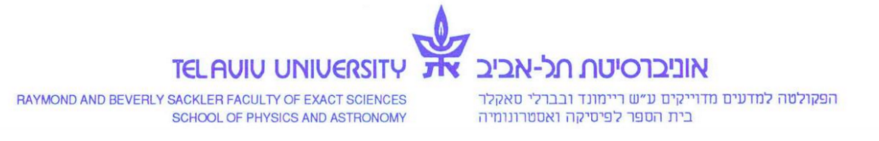
\includegraphics[scale=0.65]{figures/TAUlogo.png}\par\vspace{1cm}
	\vspace{1cm}
	{\scshape\Large Thesis Submitted In partial Fulfillment of the Requirements for the Degree of\par}
	\vspace{1cm}
	{\scshape\Large Master of Science\par}
	\vspace{1.5cm}
	{\huge\bfseries Charged Holographic Strings\par}
	\vspace{2cm}
	{\Large\itshape Lior Blech\par}
	\vfill
	{\scshape\Large Written Under the Supervision of\par
	Prof.~Jacob Sonnenschein}

	\vfill

% Bottom of the page
	{\large \today\par}
\end{titlepage}
\begin{abstract}
We revisit the holographic description of hadrons, adding an electromagnetic interaction term and taking account of one loop corrections through a casimir energy term. We first review the theoretical background: AdS/CFT correspondence, confining gravitational backgrounds and the approximating model of the spinning string with endpoint masses, including the one loop quantum corrections. We then analyse the effect of adding the electromagnetic charges and the casimir energy. Finally we confront the results with PDG data by fitting to the Regge trajectories and attempt to further constrict the parameter space through the determination of quark mass differences.
\end{abstract}

\tableofcontents

\section{Introduction}
\FloatBarrier
\subsection{Confinement and Regge Trajectories}

Confinement\cite{Greensite08} is usually defined as the apparent absence of free quarks in nature. This definition refers to the absence of free hadronic particles with fractional electric charge. Although intuitive this definition is imprecise. Suppose in nature there exists a massive scalar in the fundemental representation of $SU\left(3\right)$ and otherwise no charge. This scalar and a quark would form a bound state in the trivial representation of $SU\left(3\right)$ and fractional electric charge, albeit with a higher mass, which could be detected at a future accelarator. This kind of particle would not really qualify as a free quark, but still, it motivates us to look for a better definition.

Another possible definition would be color confinement, which states that there are no isolated particles in nature with non vanishing color charge. This definition also does not capture the essence of the problem. Suppose we introduce a higgs field in the fundemental representation of $SU\left(3\right)$ with couplings such that all gluons acquire a mass at tree level. The color charge is the integral of the electric field over a closed volume:
\begin{equation}
Q^a=\int\limits_{\partial V} \vec{E}^a \cdot d\vec{S}
\end{equation}
An isolated quark far from the boundary of the volume would thus have a color charge which is essentially zero, as the electric field would fall off exponentially with distance. So a quark viewed from a distance much greater than the inverse gluon mass would appear to be a color singlet.

What really distinguishes QCD from a gauge theory with spontaneous symmetry breaking is the fact that meson states in QCD fall on Regge trajectories, which are not found in bound state systems with coloumb or yukawa attractive forces. Regge trajectories are straight lines in the $\left(J,M^2\right)$ plane.

A simple model which was already known in the 60's \cite{Collins} to replicate the linear nature of Regge trajectories, is the spinning open relativistic string given by the Namboo-Goto action. The NG action describes the proper area of the string worldsheet:
\begin{equation}
S=T_{string}\iint \mathrm{d}^2\sigma \sqrt{-\det\left(\frac{\partial x^\mu}{\partial \sigma^a}\frac{\partial x_\mu}{\partial \sigma^b}\right)}
\end{equation}
Where $T_{string}\left[GeV^{-2}\right]$ is the string tension and
\begin{align}
&\sigma^1=\tau\in\left(-\infty,\infty\right)\\
&\sigma^2=\sigma\in\left[-\pi,\pi\right]
\end{align}
Are the worldsheet coordinates, which are affine parameters describing the worldsheet. The action is invariant upon general coordinate transformations. We choose in this case the orthogonal gauge which is defined by:
\begin{subequations}
\begin{align}
&\frac{dx^\mu}{d\tau} \frac{dx_\mu}{d\tau}=-\frac{dx^\mu}{d\sigma}\frac{dx_\mu}{d\sigma}\\
&\frac{dx^\mu}{d\sigma} \frac{dx_\mu}{d\tau}=0
\end{align}
\end{subequations}
Under which the action reduces to the more convenient form:
\begin{equation}
S=\frac{T_{string}}{2}\iint \left( \frac{dx^\mu}{d\tau} \frac{dx_\mu}{d\tau}-\frac{dx^\mu}{d\sigma} \frac{dx_\mu}{d\sigma} \right)\mathrm{d}\sigma\mathrm{d}\tau
\end{equation}
The conjugate momenta are:
\begin{equation}
P^\mu=\frac{\partial \mathcal{L}}{\partial \dot{x^\mu}}=T_{string} \eta_{\mu\nu}\dot{x}^\nu 
\end{equation}
The boundary conditions appropriate for an open string are:
\begin{subequations}
\begin{align}
&\dot{x}^0_{\sigma=\pm\pi}=const\\
&P^i_{\sigma=\pm\pi}=0
\end{align}
\end{subequations}
And the equations of motion are simply the wave equation for each coordinate:
\begin{equation}
\frac{\partial^2 {x}^\mu}{\partial \tau^2}-\frac{\partial^2 {x}^\mu}{\partial \sigma^2}=0
\end{equation}
A solution describing a spinning string is:

\begin{align}
&x^0=A\tau &x^3=\cdots=const\notag\\
&x^1=A\cos\left(\tau\right)\sin\left(\sigma\right) &x^2=A\sin\left(\tau\right)\sin\left(\sigma\right)
\end{align}

The parameter $A$ is needed in the time variable to ensure the solution is in the orthogonal gauge. We now compute the energy and angular momentum of this configuration and find the relation in the $\left(J,E^2\right)$ plane. The energy is the generator of poincare time translations and angular momentum is the generator of rotations in the poincare coordinates. The expressions are:
\begin{subequations}
\begin{align}
&E=\frac{T_{string}}{2}\int\limits_{-\pi}^{\pi} \frac{dx^0}{d\tau} \mathrm{d}\sigma  \\
&J_i=\frac{T_{string}}{2}\int\limits_{-\pi}^{\pi}\epsilon_{ijk}x_j \dot{x}^k \mathrm{d}\sigma
\end{align}
\end{subequations}

Substituting the spinning solution into these results in:
\begin{subequations}
\begin{align}
&E=\pi T_{string} A \\
&J_3=\frac{T_{string}\pi}{2}A^2
\end{align}
\end{subequations}

Finally we combine the two relations, eliminating $A$ in favor of $E$ in $J$ and get the formula for a classical linear trajectory:
\begin{equation}
\label{eq:intro-traj}
J=\frac{E^2}{2\pi T_{string}}
\end{equation}

Here we can define a quantity which we will use later, the Regge slope $\alpha'=\frac{1}{2\pi T_{string}}$. The expression \ref{eq:intro-traj} lacks another important property of Regge trajectories: the \emph{intercept}. The intercept is the result of quantum mechanical fluctuations, as will be demonstrated in section \ref{sec:Spinning Holographic Strings}. Due to this interesting result string theory was initially investigated as a theory of the strong interactions. Due to the presence of unwanted (from the strong interaction point of view) particles in the string spectrum and the discovery of asymptotic freedom, it was abandoned as a theory of the strong interactions, while continuing to develop as a fundemental theory of particle physics and gravity.

\subsection{AdS/CFT Correspondence}

In time it was discovered that apart from strings, string theory contained additional degrees of freedom, p-Branes, which are extended objects where open strings end. Furthermore, p-branes were recognized to be the same objects as D branes, which are solitonic solutions of supergravity (which is the low energy, or small slope, limit of superstring theory). Dp branes, as they are called, can also carry gauge fields which are said to "live" on their surface. Open strings then correspond to sources or sinks of flux on the brane.

The study of Dp branes and the theories that live on them led to the Maldacena conjecture that $\mathcal{N}=4$ SYM is equivalent to type IIB string theory compactified on $AdS_5\times S^5$\cite{Maldacena97,Aharony11,Vecchia98}. The conjecture relates the string theory, supergravity and gauge theory parameters:
\begin{align}
&g_{YM}^2\equiv\frac{\lambda}{N}=4\pi g_s &R_{S_5}^2=R_{AdS_5}^2=\lambda^{1/2}\alpha'
\end{align}
Where
\begin{description}
\item[$g_{YM}$] is the gauge theory coupling
\item[$\lambda$] is the t'hooft coupling
\item[N] is the number of coincident D branes as well as the type of gauge group $SU\left(N\right)$
\item[$g_s$] is the string coupling
\item[$R_{S_5}$] is the radius of the sphere
\item[$R_{AdS_5}$] is the radius of AdS
\item[$\alpha'$] is the slope parameter as defined above
\end{description}

The SYM theory lives on the boundary of AdS while the string theory lives in the bulk. The perturbative description is valid for small $g_{YM}$ while the supergravity description is valid for large radii, hence large $\lambda$ and finite $g_{YM}$. In this sense it is also a weak-strong coupling correspondence. A consequence of the correspondence must be that correlation functions in the gauge theory can be computed in the string theory by using the gauge theory operator insertions as the boundary conditions for the string theory computations. The correspondence in the generating functional is:
\begin{equation}
Z_{SYM}\left(\theta_0\right)=< e^{\int d^4x\theta_0\left(x\right)Q\left(x\right)}>
\sim Z_{stringy}\left(\theta_0\right)=\int\limits_{\theta\rightarrow\theta_0}\mathcal{D}\theta e^{-S\left[\theta\right]}
\end{equation}
Where $\theta_0\left(x\right)$ is the source of the boundary field $Q\left(x\right)$.

SYM theory is a supersymmetric version of Yang Mills theory, which turns out to be conformally invariant at the quantum level. The most powerfull evidence for the AdS/CFT correspondence is the correspondence of $SYM\mathcal{N}=4$ theory to string theory on the $AdS_5\times S_5$ background. The correspondence in this case is supported by the fact that the two theories contain the same symmetries. We will now briefly describe conformal symmetry ,supersymmetry and the symmetries of AdS space.

The Conformal symmetry group is the group of transformations which preserve the form of the metric up to an arbitrary scale factor $g_{\mu\nu}\left(x\right)\rightarrow\Omega^2\left(x\right)g_{\mu\nu}\left(x\right)$. It is generated by the poincare transformations, the scale transformations
\begin{equation}
x^\mu\rightarrow\lambda x^\mu
\end{equation}
and the special conformal transformations
\begin{equation}
x^\mu\rightarrow\frac{x^\mu+a^\mu x^2}{1+2x^\nu a_\nu+a^2x^2} 
\end{equation}
The generators of Lorentz $M_{\mu\nu}$, Translation $P_\mu$, Scale $D$ and Special Conformal $K_\mu$ transformations obey the conformal algebra:
\begin{align}
&[M_{\mu\nu},P_\rho]=-i(\eta_{\mu\rho}P_\nu-\eta_{\nu\rho}P_\mu) &[M_{\mu\nu},K_\rho]=-i(\eta_{\mu\rho}K_\nu-\eta_{\nu\rho}K_\mu) \notag \\
&[M_{\mu\nu},M_{\rho\sigma}]=-i\eta_{\mu\rho}M_{\nu\sigma}\pm\textit{permutations} &[D,K_\mu]=iK_\mu \notag \\
&[D,P_\mu]=-iP_\mu &[P_\mu,K_\nu]=2iM_{\mu\nu}-2i\eta_{\mu\nu}D & \notag \\
&[M_{\mu\nu},D]=0
\end{align}
where all other commutators vanish. This algebra is isomorphic to the algebra of $SO(d,2)$ with signature $-,+,+,\hdots,+,-$ and generators $J_{ab}$:
\begin{align}
&J_{\mu\nu}=M_{\mu\nu} &J_{\mu d}=\frac{1}{2}(K_\mu-P_\mu) &J_{\mu(d+1)}=\frac{1}{2}(K_\mu+P_\mu) &J_{(d+1)d}=D \\
&\mu,\nu=0,1,\hdots,d-1 \notag
\end{align}

The supersymmetry transformation is generated by a fermionic operators $Q$ which anti-commutes with the translation operators $P_\mu$. For some numbers of dimensions and supersymmetry generators it is possible to join the supersymmetry and conformal group into one simple group. These superconformal algebras exist only for $d\leq 6$. In these algebras there arise two more types of generators: the fermionic $S$ and the bosonic $R$ R-symmetry. The algebra is schematically:
\begin{align}
&[D,Q]=-\frac{i}{2}Q & [D,S]=\frac{i}{2}S &[K,Q]\approx S &[P,S]\approx Q \notag \\
&{Q,Q}\approx P &{S,S}\approx K &{Q,S}\approx M+D+R
\end{align}

The $p+2$ dimensional $Ads_{p+2}$ can be represented as the hyperboloid
\begin{equation}
X_0^2+X_{p+2}^2-\sum_{i=1}^{p+1}X_i^2=R^2
\end{equation} 
in the flat $p+3$ dimensional space with metric
\begin{equation}
ds^2=-dX_0^2-dX_{p+2}^2+\sum_{i=1}^{p+1}dX_i^2
\end{equation}
This space has the isometry $SO(2,p+1)$ by construction and it is homogeneous and isotropic. A useful set of coordinates $(u,t,\vec{x})$, called the poincare coordinates, is defined by the relations:
\begin{align}
&X_0=\frac{1}{2u}\left(1+u^2 \left(R^2+\vec{x}^2-t^2\right)\right) &X_{p+2}=Rut \notag \\
&X^i=Rux^i \qquad \left(i=1,\hdots,p\right) \notag \\
&X^{p+1}=\frac{1}{2u}\left(1-u^2 \left(R^2-\vec{x}^2+t^2\right)\right)
\end{align}
In these coordinates the metric is:
\begin{equation}
ds^2=R^2\left(\frac{du^2}{u^2}+u^2\left(-dt^2+d\vec{x}^2\right)\right)
\end{equation}
The metric is manifestly poincare invariant ($ISO\left(1,p\right)$). Also the transformation $SO\left(1,1\right)$ defined by:
\begin{equation}
\left(t,\vec{x},u\right)\rightarrow \left(ct,c\vec{x},c^{-1}u\right)\qquad c>0
\end{equation}
is an isometry of the space. This transformation is identified with the dilatation $D$ in the conformal symmetry group of $\mathbb{R}^{1,p}$. Thus $AdS_{p+2}$ has the same number of symmetries as a conformal theory in flat space with $p+1$ dimensions.

Lastly the $SO\left(2,p+1\right)$ isometry group of $AdS_{p+2}$ has a supersymmetric generalization called an \textit{AdS} supergroup, and it turns out that \textit{AdS} space preserves as many supersymmetries as flat space.

The exact matching between the superconformal algebra of $SYM\mathcal{N}=4$ and the isometry group of supergravity (and thus low energy string theory) on $AdS_5\times S_5$ provides the strongest evidence for the maldacena correspondence.
%The origin of string theory can be traced back to the 60's. Physicists have tried to make sense of many of the strong interactions experimental data. There were many particles and resonances detected, and there was no satisfactory theory to incorporate them. Some regularities were observed. The first was the duality of the four point amplitudes in the \textbf{s} and \textbf{t} channels. The second observation was that the energy and the angular momentum of some particles could be placed on straight lines: $J=\alpha'm^2+a$. These lines are called Regge Trajectories. A suitable scattering amplitude for two by two*******

\FloatBarrier
\subsection{Confining Backgrounds}
As has been mentioned, the Maldacena correspondence allows us to compute strong coupling quantities in gauge theories. This has given hope that a string theory dual to QCD might be found which would enable us to handle the nonperturbative regime. The fact that string models describe well the Regge trajectories gives further motivation. While this has not been accomplished to date, there has been progress in that direction.

Using the gauge-gravity duality, supergravity backgrounds have been constructed that are dual to confining gauge theories. To deal with non supersymmetric gauge dynamics one makes use of Witten's method \cite{Witten98,Kuperstein04} of  using compact euclidian time with anti-periodic boundary conditions. We investigate whether the stringy picture in a confining background can reproduce the properties of real hadrons by fitting to regge trajectories and predict hadron electromagnetic mass differences. This section summarizes the results of previous works on what kinds of backgrounds confine.  

\FloatBarrier
\subsubsection{Stringy Wilson Loop}
In gauge theories the operators called wilson lines (or loops) are gauge invariant operators defined by
\begin{equation}
W\left(C\right)=\frac{1}{N}\emph{TrP} e^{i\oint\limits_CA_\mu \dot{x}^\mu\left(\tau\right)\mathrm{d}\tau }
\end{equation}
The energy of a quark anti-quark pair can be extracted from the infinite strip wilson loop by the relation \cite{Sonnenschein00}:
\begin{equation}
\left\langle W\left(C\right)\right\rangle=A\left(L\right)e^{-TE\left(L\right)}
\end{equation}

\begin{tikzpicture}
\draw[color=red] (-1.5,-2.5) rectangle (1.5,2.5);
\draw[<->,dashed] (-1.5,2.6) -- node[anchor=south,near end] {L} (1.5,2.6);
\draw[<->,dashed] (1.7,-2.5) --node[anchor=west,near end] {T} (1.7,2.5);
\draw[->] (-2,0) -- (2,0) node[anchor=west] {x};
\draw[->] (0,-3) -- (0,3) node[anchor=south] {t};
\end{tikzpicture}

Where \emph{T} is the time extension of the loop. In the AdS/CFT correspondence, the stringy dual of the wilson line is the Nambu-Goto string \cite{Maldacena98}.
\begin{equation}
\left\langle W\left(C\right)\right\rangle\sim e^{-S_{NG}}
\end{equation}
So that
\begin{equation}
S_{NG}=TE\left(L\right)
\end{equation}
We analyse wilson loops inside a d dimensional space-time with the metric \cite{Kinar99}
\begin{equation}
ds^2=-G_{00}\left(s\right)dt^2+G_{||}\left(s\right)dx_{||}^2+G_{ss}\left(s\right)ds^2+G_{TT}\left(s\right)dx_T^2
\end{equation}
where the $x_{||}$ are p space coordinates on a $D_p$ brane and \textbf{s} and $x_T$ are radial coordinates and transverse directions respectively. For string configurations which are static and approximately stretch only along the radial and one $x_{||}$ directions we can take the gauge $t=\tau, x_{||}=x$. The induced worldsheet metric then takes the form:
\begin{equation}
h=
\begin{pmatrix}
-G_{00}	& 0 \\
0		& G_{||}+G_{ss}\left(\partial_{x}s\right) \\ 
\end{pmatrix}
\end{equation} 
The corresponding Nambu Goto action is
\begin{equation}
S_{NG}=T\int\sqrt{f^2\left(s\left(x\right)\right)+g^2\left(s\left(x\right)\right)\left(\partial_xs\right)^2}\mathrm{d}x
\end{equation}
Where $T=\int\mathrm{d}t$ and we made the following substitutions:
\begin{subequations}
\begin{align}
&f^2\left(s\left(x\right)\right)=G_{00}\left(s\left(x\right)\right)G_{||}\left(s\left(x\right)\right)\\
&g^2\left(s\left(x\right)\right)=G_{00}\left(s\left(x\right)\right)G_{ss}\left(s\left(x\right)\right)
\end{align}
\end{subequations}
Notice that \textbf{x} does not appear explicitly in the action and so there is a conserved current:
\begin{align}
&\frac{\partial L_{NG}}{\partial \left(ds/dx\right)}\frac{ds}{dx}-L_{NG}=const \notag \\
&=\cdots=-\frac{f^2\left(s\left(x\right)\right)}{\sqrt{f^2\left(s\left(x\right)\right)+g^2\left(s\left(x\right)\right)\left(\partial_xs\right)^2}}=const=-K
\end{align}
For $\frac{ds}{dx}|_{s_0}=0$ we get $f\left(s_0\right)=K$. Using this and extracting $\frac{ds}{dx}$ we get:
\begin{equation}
\frac{ds}{dx}=\pm\frac{f\left(s\right)}{g\left(s\right)} \frac{\sqrt{f^2\left(s\right)-f^2\left(s_0\right)}}{f\left(s_0\right)}
\end{equation}
The picture is of the string stretching down from the boundary $s\rightarrow\infty$ down to $s\rightarrow s_0$ where it is horizontal, and back into the boundary. The seperation distance between the string endpoints (quark anti quark) is
\begin{equation}
\label{eq:stringseperation}
L=\int dx=2\int\limits_{s_0}^{\infty} \frac{g\left(s\right)}{f\left(s\right)} \frac{f\left(s_0\right)}{\sqrt{f^2\left(s\right)-f^2\left(s_0\right)}} \mathrm{d}s
\end{equation}
We can use the two relations to calculate the action and extract the quark potential $E=\frac{S_{NG}}{T}$
\begin{align}
S_{NG}&=2T\int\limits_{s_0}^{\infty} \frac{g\left(s\right)}{f\left(s\right)} \frac{f\left(s_0\right)}{\sqrt{f\left(s\right)^2-f\left(s_0\right)^2}} \sqrt{f\left(s\right)^2+g\left(s\right)^2\frac{f\left(s\right)^2}{g\left(s\right)^2} \frac{f\left(s\right)^2-f\left(s_0\right)^2}{f\left(s_0\right)^2}}\mathrm{d}s \notag \\
&=2T\int\limits_{s_0}^{\infty} \frac{g\left(s\right)f\left(s\right)}{\sqrt{f\left(s\right)^2-f\left(s_0\right)^2}}\mathrm{d}s=\infty
\end{align}
The action diverges because of the infinite extent of the string. In order for the string length to converge the slope $\frac{ds}{dx}$ has to diverge on the boundary. This implies $f\left(s\right)\gg f\left(s_0\right)$ on the boundary. In this region the string is vertical and the energy density there is approximately just $g\left(s\right)$. In that case we can renormalize the action by
\begin{itemize}
\item[(a)] regularizing the integral $\int\limits_{s_0}^{\infty} \rightarrow \int\limits_{s_0}^{s_1}$
\item[(b)] substracting the quark masses defined by
\end{itemize}
\begin{equation}
m_q=\int\limits_{0}^{s_1}g\left(s\right)\mathrm{d}s
\end{equation}
The renormalized quark antiquark potential is now
\begin{equation}
V=f\left(s_0\right)L+2\int\limits_{s_0}^{s_1} \frac{g\left(s\right)}{f\left(s\right)}\left(\sqrt{f\left(s\right)^2-f\left(s_0\right)^2}-f\left(s\right)\right)\mathrm{d}s-2\int\limits_{0}^{s_0}g\left(s\right)\mathrm{d}s
\end{equation}
A sufficient condition for confinement found in \cite{Sonnenschein00,Kinar98} is if either:
\begin{itemize}
\item f has a minimum at $s_{min}$ and $f\left(s_{min}\right)\neq0$.
\item g diverges at $s_{div}$ and $f\left(s_{div}\right)>0$.
\end{itemize}
The first condition asserts that the potential contains a linear term. Also under this condition there must be a region where $f\left(s\right)\gg f\left(s_0\right)$. In the case of a divergence of $g\left(s\right)$,
\begin{equation}
\frac{ds}{dx}|_{s=s_{div}}=\pm\frac{f\left(s\right)}{g\left(s_{div}\right)} \frac{\sqrt{f^2\left(s\right)-f^2\left(s_0\right)}}{f\left(s_0\right)}=0
\end{equation}
So that a string long enough to reach $s_{div}$ stretches horizontaly along $s=s_{div}$ for much of its length. So the stringy picture in a confining background is that of two strings stretching verticaly from the boundary down to either the "wall" $s=s_{div}$ or down to $s_0$ where $f$ has a minimum, and connecting horizontaly.

An example is that of the dual model of pure YM in d=3 \cite{Kinar98}:
\begin{subequations}
\label{eq:YM dual}
\begin{align}
&L_{NG}=\sqrt{\left(\frac{U}{R}\right)^4+\left(U'\right)^2\left(1-\left(\frac{U_T}{U}\right)^4\right)^{-1}} \\
&V=\frac{U_T^2}{2\pi R^2}L-2\kappa+O\left(\left(\log L\right)^\beta e^{-\alpha L}\right)
\end{align}
\end{subequations}

\begin{figure}
\centering
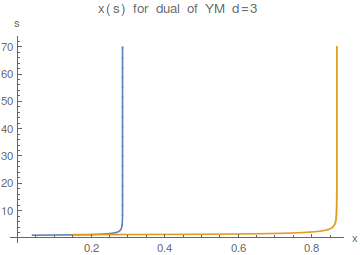
\includegraphics[scale=0.7]{figures/stringConfiguration.png}
\caption{String configurations of the YM dual \ref{eq:YM dual} with $s_{div}=R=1$. The blue and orange strings differ in the overal string length, controlled through the dependnce on $s_0$ \ref{eq:stringseperation}. It can be observed that the length of the transition region between horizontal and vertical sections does not scale with the string length.}
\end{figure}

This has confining behaviour and $S_{div}=U_T$. In other words to get confinment we introduce a scale in the radial direction. The wilson loop in a confining background behaves similarily to a string in flat space time, due to the U shape and the cancelation of the action of the vertical segments.

%\begin{tikzpicture}[rounded corners=2pt,scale=2]
%\draw (-16pt,0) rectangle (16pt,-15pt);
%\shade (0,0) ellipse [x radius=20pt,y radius=6pt];
%\end{tikzpicture}
\FloatBarrier
\subsubsection{From Wilson Lines To Dynamical Mesons}

In the preceding section we discussed the stringy decription of the wilson line. The quarks there were actually infinitly massive due to the strings stretching all the way to the boundary. We can introduce dynamical quarks by introducing a set of $N_f$ "flavor" Dp branes in the bulk, in addition to the stack of ($N_c$) "color" branes which lie at the boundary. Strings which stretch between the color branes and the flavor branes map to bifundemental "quarks" that transform as the $(N_c,N_f)$ representation of the $U(N_c)\times U(N_f)$ gauge symmetry. For $N_c\gg N_f$ the backreaction of the flavor branes can be ignored and the $U(N_f)$ can be treated as a global symmetry.

\begin{table}
\centering
\begin{tabular}{ l *{10}{c}}
 	& 0 & 1 & 2 & 3 & (4) & 5 & 6 & 7 & 8 & 9 \\
$D4$	 & $\circ$ & $\circ$ & $\circ$ & $\circ$ & $\circ$ &  &  &  &  & \\
$D8-D\bar{8}$	& $\circ$ & $\circ$ & $\circ$ & $\circ$ &  & $\circ$ & $\circ$ & $\circ$ & $\circ$ & $\circ$
\end{tabular}
\caption{The Sakai-Sugimoto model brane configuration. The dimension $x^4$ is compactified on a circle.}
\label{tab:Sakai-Sugimoto}
\end{table}

We use the Sakai-Sugimoto model \cite{Sakai04} which consists of $N_c$ $D4$ branes and $N_f$ $D8-D\bar{8}$ branes. The dimensions the branes extend along are described in table \ref{tab:Sakai-Sugimoto}. The $x^4$ coordinate is compactified with boundary conditions which kill supersymmetry and introduces confinement. The flavor branes in the $D4$ background are described by the embedding $x^4\left(U\right)$ where $U$ is the radial direction away from the $D4$ brane (with the $D4$ brane residing at $U=\infty$). In their analysis Sakai and Sugimoto determined that the $D8-D\bar{8}$ branes hang from the $D4$ brane and meet at  some $U$, forming a single brane and spontaneously breaking the chiral symmetry $U\left(N_f\right)_L\times U\left(N_f\right)_R\rightarrow U\left(N_f\right)$. One can seperate the flavor branes in the radial $U$ direction, further breaking the flavor symmetry.

\begin{figure}
\centering
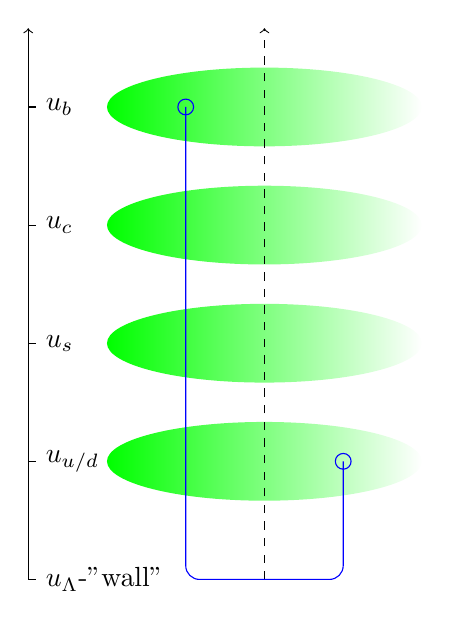
\begin{tikzpicture}[rounded corners=5pt,scale=0.1]
\shade[left color=green,right color=white] (30,15) ellipse [x radius=20,y radius=5];
\shade[left color=green,right color=white] (30,30) ellipse [x radius=20,y radius=5];
\shade[left color=green,right color=white] (30,45) ellipse [x radius=20,y radius=5];
\shade[left color=green,right color=white] (30,60) ellipse [x radius=20,y radius=5];
\draw[dashed,->] (30,0) -- (30,70);
\draw[->] (0,0) -- (0,70);
\draw[color=blue] (20,60) circle [radius=1,fill=blue]--(20,0)--(40,0)--(40,15) circle [radius=1,fill=blue];
\draw (0,0)--(1,0) node[anchor=west] {$u_\Lambda$-"wall"};
\draw (0,15)--(1,15) node[anchor=west] {$u_{u/d}$};
\draw (0,30)--(1,30) node[anchor=west] {$u_s$};
\draw (0,45)--(1,45) node[anchor=west] {$u_c$};
\draw (0,60)--(1,60) node[anchor=west] {$u_b$};
\end{tikzpicture}
\caption{Illustration of flavor probe branes. Each brane is located at a different radial coordinate which determines the mass of the corresponding quark flavor.}
\end{figure}

Now instead of starting and ending on the boundary the strings can start and end on the flavor branes. A string would now have an endpoint mass:
\begin{equation}
m_q=	T\int\limits_{s_0}^{s_f} \sqrt{G_{00}G_{ss}}\mathrm{d}s
\end{equation}
Where $s_f$ is the radial coordinate of a flavor brane. In \cite{Kruczenski05} it was found that the dynamics of the open string spinning in the confining background could be described by the model of the spinning string in flat space loaded with masses at its' ends. This approximation is valid as long as the string is sufficiently long and stretches along the wall.

We have seen that it is possible to get a string theory which is dual to a confining gauge theory with flavor symmetries and fundemental quarks and the states dual to mesons are spinning strings stretching between the flavor branes. In \cite{Seki08} a similiar analysis was carried out for baryons, which were found to be described by spinning strings which at one end connect with a flavor brane and at the other end with a baryonic vertex, which then connects with two other short strings which in turn connect to flavor branes. The baryonic vertex is itself a D5 brane wrapped around the $S_5$. In addition we see that this theory can be analysed through the approximation of the spinning string with masses at the endpoints. This approximation lies at the heart of the present work.

\FloatBarrier
\subsection{Spinning Holographic Strings}
\label{sec:Spinning Holographic Strings}

In the previous section we have seen that strings in gravitational backgrounds which connect with probe branes can be approximately described as strings in flat spacetime, with endpoint masses proportional to the length of the horizontal string sections. This section will present the results obtained in the analysis of such a model and use them to discuss the general approach to the holographic string problem.

The model of the spinning string with massive endpoints is described using the Nambu-Goto action and relativistic point particle action:

\begin{align}
\label{eq:actionmassive}
S&=-T\iint\limits_{(0,-l_{2})}^{(T,l_{1})}\mathrm{d}^{2}\sigma\sqrt{-\det h}-m_1\int\limits_{0}^{T}\mathrm{d}\tau\sqrt{u^{\mu}u_{\mu}}|^{\sigma=l_{1}}-m_2\int\limits_{0}^{T}\mathrm{d}\tau\sqrt{u^{\mu}u_{\mu}}|^{\sigma=-l_{2}}=\notag\\
&=-T\iint\limits_{(0,-l_{2})}^{(T,l_{1})}\mathrm{d}^{2}\sigma\sqrt{-\det h}-m\int\limits_{0}^{T}\mathrm{d}\tau\sqrt{u^{\mu}u_{\mu}}|_{\sigma=-l_{2}}^{\sigma=l_{1}}
\end{align}

The endpoint masses (pointlike massive particles) are located at the coordinates specified by $\sigma=l_1,-l_2$, and the masses are allowed to vary between the two ends. The second line of equation \ref{eq:actionmassive} shows an example of a shorthand we use to write the two point-particle actions as one.

In section \ref{sec:eom} we show how to derive the equations of motion, energy and angular momentum for the case of the charged holographic string discussed there. For now we simply write down the results obtained in \cite{Sonnenschein14} for the case of identical endpoint masses.

\begin{subequations}
\begin{align}
&\text{The equation of motion is:}\notag\\
&\gamma\beta m \omega-\frac{T}{\gamma}=0\\
&\text{The energy is:}\notag\\
&E=\frac{2T}{\omega}\sin^{-1}\left(\beta\right)+2m\gamma\\
&\text{The angular momentum is:}\notag\\
&J=T\frac{-\frac{\beta}{\gamma}+\sin^{-1}\left(\beta\right)}{\omega^{2}}+2m\frac{\gamma\beta^{2}}{\omega}
\end{align}
\end{subequations}

Where:
\begin{itemize}
\item[c]=1.
\item[$\beta$] is the velocity of the endpoints.
\item[$\gamma$]$=\frac{1}{\sqrt{1-\beta^2}}$
\item[$T$] is the string tension.
\item[$\omega$] is the rate of rotation, such that $\beta=\omega l$ and $l$ is the distance of each endpoint to the center of rotation.
\end{itemize}

Notice that the equation of motion can be used to relate the rate of rotation with the velocity:
\begin{equation}
\label{eq:omega}
\omega=\frac{T}{m\gamma^2\beta}
\end{equation}
So putting this back in the expressions for the energy and angular momentum results in:

\begin{subequations}
\begin{align}
&E=2m\gamma^2\beta\sin^{-1}\left(\beta\right)+2m\gamma\\
&J=m^2\gamma^4\beta^2 \frac{-\frac{\beta}{\gamma}+\sin^{-1}\left(\beta\right)}{T}+\frac{2m^2\gamma^3\beta^{3}}{T}
\end{align}
\end{subequations}

We are interested in the predicted regge trajectories in the limits of small and large quark mass, which corresponds to $\beta\rightarrow1$ and $\beta\rightarrow0$ respectively (this results from equation \ref{eq:omega}, assuming constant string tension and rotation rate).The procedure to get the expression for the regge trajectory in each limit  is:
\begin{enumerate}
\item Expand the energy and angular momentum in a taylor series around the corresponding limit.
\item Find the inverse series for the energy $\beta\left(E\right)$ \cite{WolframSeriesReversion}.
\item Plug $\beta\left(E\right)$ into the angular momentum series and get $J\left(E\right)$.
\end{enumerate}

The resulting series are:

\begin{subequations}  
\begin{align}
&\text{Light quark limit }\beta\rightarrow1\notag\\
&J=\alpha' E^2-\frac{8 \sqrt{\pi } \alpha' m^{3/2}}{3}\sqrt{E}+\frac{2}{5}\frac{\pi^{3/2}m^{5/2}\alpha'}{\sqrt{E}}+\hdots \\
&\text{Heavy quark limit }\beta\rightarrow0\notag\\
&J=\frac{4\pi\alpha'\sqrt{m} \left(E-2 m\right)^{3/2}}{3\sqrt{3}}+\frac{7\pi\alpha'  \left(E-2m\right)^{5/2}}{54\sqrt{3}\sqrt{m}}+\hdots
\end{align}
\end{subequations}

Here we have defined the string 'slope' related to the string tension by:
\begin{equation}
\alpha'=\frac{1}{2\pi T}
\end{equation}

Observe that in the light quark limit the regge trajectory reduces to the linear trajectory of the spinning string with no endpoint masses $J=\alpha'E^2$. This trajectory still does not predict an intercept. In \cite{Sonnenschein14} the intercept has been introduced by taking
\begin{equation}
J\rightarrow J-a
\end{equation}
and the fits to the regge trajectories of various hadrons have been made.

The intercept is created by the quantum mechanical zero point energy. This energy is also called a casimir energy because in the casimir effect it is the energy difference induced by this energy term causes the  observed casimir force. In \cite{Lambiase96} the quantum corrections to the energy of the massive stationary string have been calculated. There it can be seen that the hamiltonian for the stationary string is reduced to:
\begin{equation}
H=\sum_{n=1}^{\infty}\sum_{j=1}^{D-2}\omega_na_n^{j\dagger}a_n^j+TR+\frac{D-2}{2}\sum_{n=1}^\infty \omega_n+\sum_{i=1,2} m_i
\end{equation}

Where the eigenfrequencies $\omega_n$ satisfy:
\begin{equation}
\tan\left(\omega_nR\right)=\frac{2mTR\left(\omega_nR\right)}{m^2\omega_n^2R^2-T^2R^2}
\end{equation}
Where $R$ is the string length and $D$ is the number of spacetime dimensions, so that the energy in terms of the dimensionless quantity $\Omega_n=\omega_n R$ is:

\begin{equation}
H=\frac{1}{R}\sum_{n=1}^{\infty}\sum_{j=1}^{D-2}\Omega_n a_n^{j\dagger}a_n^j+TR+\frac{D-2}{2R}\sum_{n=1}^\infty \Omega_n+\sum_{i=1,2} m_i
\end{equation}

Therefore the string potential is

\begin{equation}
\label{eq:stringpotential}
V\left(R\right)=TR+\frac{D-2}{2R}\sum_{n=1}^\infty \Omega_n
\end{equation}
So we see that the string introduces both a confining linear potential and a $1/R$ term.This term is the generalization of the famous Luscher term. In the case of the string with massive endpoints it turns out this additional potential is attractive, similar to the luscher result, but has mass and string length dependent corrections. This leads us to guess that the quantum correction to the spinning holographic string can be made by introducing a casimir energy term of the same form with some free parameter which stands in for the sum $\sum_{n=1}^\infty \Omega_n$.

In \cite{Sonnenschein14} the charges of the quarks have not been taken account of. The charges are expected to contribute to observables such as the mass differences between different hadrons, as well as decay rates and magnetic and electric dipoles. In the next section we will add the point charges and take the same philosophy: calculate the classical trajectory and add the quantum corrections by hand (although a bit differently).

\FloatBarrier
\section{Charged Holographic Strings}

The strings in our model attach to stacks of $N_f$ flavor branes. As such they are charged under the gauge group $SU(N_f)$. If the flavor branes are seperated this gauge group gets broken spontaneously down to a number of $U(1)$ gauge groups, which is just the electromagnetic interaction. In our model we take account of the electromagnetic interaction by associating electric charge with the string endpoints. We now present the formulation and analyze the model.

\FloatBarrier
\subsection{The Action}

We add charges to the end points by considering the action from the previous section and adding two electromagnetic interaction lagrangians at the endpoints. Note that instead of using the Namboo-Goto action for the string one can use the polyakov action, and similarily the point particles can be described by the alternative action quadratic in the coordinates. We use here the choice of a namboo goto action for the string and a "proper interval" action for the point masses:

\begin{equation}
S=-T\iint\limits_{(0,-l_{2})}^{(T,l_{1})}\mathrm{d}^{2}\sigma\sqrt{-\det h}-m\int\limits_{0}^{T}\mathrm{d}\tau\sqrt{u^{\mu}u_{\mu}}|_{\sigma=-l_{2}}^{\sigma=l_{1}}-q\int\limits_{0}^{T}u^{\mu}A_{\mu}\mathrm{d}\tau|_{\sigma=-l_{2}}^{\sigma=l_{1}}
\end{equation}

The field lagrangian density for the electromagnetic fields is not included to avoid divergent self energy terms .Instead, the electromagnetic potentials and fields are determined directly by the Lienard-Wichert formulas. The worldsheet metric is as usual:

\begin{equation*}
h=
\begin{pmatrix}
\frac{dx^{\mu}}{d\tau}\frac{dx_{\mu}}{d\tau} & \frac{dx^{\mu}}{d\tau}\frac{dx_{\mu}}{d\sigma}\\
\frac{dx^{\mu}}{d\tau}\frac{dx_{\mu}}{d\sigma} & \frac{dx^{\mu}}{d\sigma}\frac{dx_{\mu}}{d\sigma}\end{pmatrix}
\end{equation*} 

We can write for short \begin{align*}
&V^{\mu}=\cfrac{dx^{\mu}}{d\sigma} & u^{\mu}=\cfrac{dx^{\mu}}{d\tau} \\
&h=\left(\begin{array}{cc} u^{2} & u\cdot V\\ u\cdot V & V^{2} \end{array}\right)
\end{align*} 

The action can be writen then as:

\begin{equation}
S=-T\iint\limits_{(0,-l_{2})}^{(T,l_{1})}\mathrm{d}^{2}\sigma\sqrt{\left(u\cdot V\right)^{2}-u^{2}V^{2}}-m\int\limits_{0}^{T}\mathrm{d}\tau\sqrt{u^{\mu}u_{\mu}}|_{\sigma=-l_{2}}^{\sigma=l_{1}}-q\int\limits_{0}^{T}u^{\mu}A_{\mu}\mathrm{d}\tau|_{\sigma=-l_{2}}^{\sigma=l_{1}} 
\end{equation}
 
We use the static gauge where:
\begin{equation}
\label{eq:staticqauge}
t=\tau \qquad r=\sigma
\end{equation}
The 4 velocity in this gauge is
\begin{align*}
u^{\mu}&=\left(\frac{dt}{d\tau},\frac{dx}{d\tau},\frac{dy}{d\tau},\frac{dz}{d\tau}\right)
=\left(1,\sigma\frac{d\cos\left(\theta\right)}{d\tau},\sigma\frac{d\sin\left(\theta\right)}{d\tau},0\right)=\\
&=\left(1,-\sigma\dot{\theta}\sin\left(\theta\right),\sigma\dot{\theta}\cos\left(\theta\right),0\right)
\end{align*}

The basis vectors for polar coordinates are
\begin{align*}
&\hat{r}=\cfrac{1}{r}\left(x\hat{x}+y\hat{y}\right) & \hat{\theta}=\cfrac{1}{r}\left(x\hat{y}-y\hat{x}\right)
\end{align*}
The components for $ A^{\mu} $ in polar coordinates are thus:
%\begin{equation*}
%u^{0}=1
%\end{equation*}
%\begin{equation*}
%u^{r}=\vec{u}\cdot\hat{r}=\cfrac{1}%{\sigma}\left(-\sigma^{2}\dot{\theta}sin\left(\theta\right)cos\left(\theta\right)
%+\sigma^{2}\dot{\theta}sin\left((\theta\right)cos\left(\theta\right)\right)=0
%\end{equation*}

%\begin{align*}
%u^{\theta}&=
%\vec{u}\cdot\hat{\theta}=
%\left(
%\hat{t}
%-\sigma\dot{\theta}\sin\left(\theta\right)\hat{x}
%+\sigma\dot{\theta}\cos\left(\theta\right)\hat{y}\right)\cdot\cfrac{1}{r}\left(x\hat{y}
%-y\hat{x}
%\right)= \\
%&=\sigma\dot{\theta}\left(y\sin\left(\theta\right)+x\cos\left(\theta\right)\right)\cdot\cfrac{1}{\sigma}=\sigma\dot{\theta}\cfrac{1}{\sigma}\left(\sigma sin^{2}\left(\theta\right)+\sigma cos^{2}\left(\theta\right)\right)=\\
%&=\dot{\theta}\sigma
%\end{align*}
\begin{align*}
&A^{r}=\vec{A}\cdot\hat{r}=\cfrac{xA^{x}+yA^{y}}{\sigma}=cos\left(\theta\right)A^{x}+sin\left(\theta\right)A^{y}\\
&A^{\theta}=\vec{A}\cdot\hat{\theta}=\cfrac{-yA^{x}+xA^{y}}{\sigma}=-sin\left(\theta\right)A^{x}+cos\left(\theta\right)A^{y}
\end{align*}
Which can be recognized as a rotation by angle $\theta$. The inverse transformation is then:
\begin{align*}
&A^{x}=cos\left(\theta\right)A^{r}-sin\left(\theta\right)A^{\theta}\\
&A^{y}=sin\left(\theta\right)A^{r}+cos\left(\theta\right)A^{\theta}
\end{align*}

The product-sum $ u^{\mu}A_{\mu} $ in our gauge is then:
\begin{align*}
u^{\mu}A_{\mu}&=u^{t}A^{t}-u^{x}A^{x}-u^{y}A^{y}-u^{z}A^{z}=\\
&=A^{t}+\sigma\dot{\theta}sin\left(\theta\right)\left(cos\left(\theta\right)A^{r}-sin\left(\theta\right)A^{\theta}\right)
-\sigma\dot{\theta}cos\left(\theta\right)\left(sin\left(\theta\right)A^{r}
+cos\left(\theta\right)A^{\theta}\right)=\\
&=A^{t}-\sigma\dot{\theta}A^{\theta}
\end{align*}

Putting everything into the action, it becomes:

\begin{equation}
\label{eq:actiongauged}
S=-T\iint\limits_{(0,-l_{2})}^{(T,l_{1})} \mathrm{d}\sigma  \mathrm{d}t\sqrt{1+\sigma^{2}\left(\theta'^{2}-\dot{\theta}^{2}\right)}-m\int\limits_0^T  \mathrm{d}t\sqrt{1-\sigma^{2}\dot{\theta}^{2}}|_{\sigma=-l_{2}}^{\sigma=l_{1}}-q\int\limits_{0}^{T}\left(A^{t}-\sigma\dot{\theta}A^{\theta}\right) \mathrm{d}	t|_{\sigma=-l_{2}}^{\sigma=l_{1}}
\end{equation}

\FloatBarrier
\subsection{Spinning String Ansatz}
Throughout our analysis we will assume the string to be rotating with a constant angular velocity. In the static gauge \ref{eq:staticqauge} this amounts to setting $\dot{\theta}=\omega$. More explicitly we have
\begin{subequations}
\label{eq:SpinningStringAnsatz}
\begin{align}
&x=\left(\tau,\sigma\cos\left(\omega\tau\right),\sigma\sin\left(\omega\tau\right)\right) \\
&\text{And for the second end point}\notag\\
&x_{opposite}=\left(\tau,\sigma\cos\left(\omega\tau+\pi\right),\sigma\sin\left(\omega\tau+\pi\right)\right)
\end{align}
\end{subequations}

\FloatBarrier
\subsection{Electromagnetic Fields}

The Lienard-Wichert formulas for the fields of a point charge are \cite{Jackson}:

\begin{subequations}
\begin{align}
&\theta\left(\vec{x},t\right)=\left[\cfrac{e}{\left(1-\vec{\beta}\cdot\vec{n}\right)R}\right]_{ret}\\
&\vec{A}\left(\vec{x},t\right)=\left[\cfrac{e\vec{\beta}}{\left(1-\vec{\beta}\cdot\vec{n}\right)R}\right]_{ret}\\
&\vec{E}\left(\vec{x},t\right)=\left[e\cfrac{\vec{n}-\vec{\beta}}{\gamma^{2}\left(1-\vec{\beta}\cdot\vec{n}\right)^{3}R^{2}}+\cfrac{e}{c}\cfrac{\vec{n}\times\left\{ \left(\vec{n}-\vec{\beta}\right)\times\dot{\vec{\beta}}\right\} }{\left(1-\vec{\beta}\cdot\vec{n}\right)^{3}R}\right]_{ret}\\
&\vec{B}\left(\vec{x},t\right)=\left[\vec{n}\times\vec{E}\right]_{ret}
\end{align}
\end{subequations}
Where 
\begin{itemize}
\item $\vec{\beta} $ is the velocity of the point charge source, divided by c.
\item $\gamma=\left(1-\beta^{2}\right)^{-1/2}$
\item $\vec{n}$ is the unit vector from the source to the point where we evaluate the fields.
\item $R$ is the distance from the source to the point where we evaluate the fields.
\item $e$ is the charge of the source.
\item $R_{ret}$ denotes the distance from the source at retarded time to the point where we evaluate the fields.
\item The formulas are evaluated with the retardation condition (also called the light cone condition) $t-t_{ret}=R_{ret}$
\end{itemize}
\begin{figure}[h]
\centering
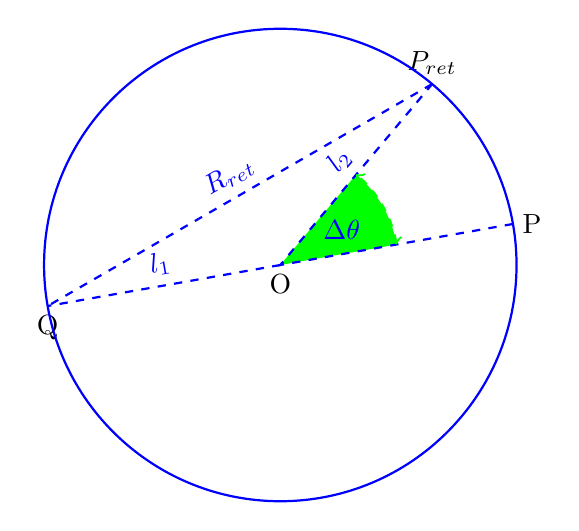
\begin{tikzpicture}[scale=0.75]

\coordinate (PP) at (50:4);
\coordinate (P) at (10:4);
\coordinate (O) at (0,0);
\coordinate (Q) at (190:4);
\draw (P) node[anchor=west] {P};
\draw (PP) node[anchor=south] {$P_{ret}$};
\draw (Q) node[anchor=north] {Q};
\draw (O) node[anchor=north] {O};

\draw[thick,blue] (O) circle [radius=4];
\draw[dashed,thick,blue] (O) --node[sloped,above]{$l_1$}(Q);
\draw[dashed,thick,blue] (PP) --node[sloped,above]{$R_{ret}$}(Q);
\draw[dashed,thick,blue] (P)--(O)--node[sloped,above]{$l_2$}(PP) pic[draw=green,fill=green,<->,angle radius=1.5cm,"$ \Delta\theta $"] {angle= P--O--PP};
\end{tikzpicture}
\caption{The geometry of the system. The points $Q$,$P$ and $P_{ret}$ are the "recieving" particle, the emmiting particle and the position of the emmiting particle at retarded time, respectively. $\Delta\theta$ is the so called retardation angle. $l_1$ and $l_2$ are the respective radii of rotation and $R_{ret}$ is the retarded distance.}
\label{fig:geometry}
\end{figure}

We will see shortly that the key quantities will be the velocities of the quarks $\beta_1$ ,$\beta_2$ and  the retardation angle $\Delta\theta$ defined in figure \ref{fig:geometry}. Looking at figure \ref{fig:geometry} we can use the cosine law to relate the retardation angle with the retarded distance $R_{ret}$:
\begin{equation*}
R_{ret}^2=l_1^2+l_2^2-2l_1l_2\cos\left(\pi-\Delta\theta\right)
\end{equation*} 
By the definitino of the retarded time, it is both ($c=1$):
\begin{itemize}
\item The time it takes the light signal to get from $P_{ret}$ to $Q$. $t-t_{ret}=R_{ret}$
\item The time it takes the emmiting particle to get from $P_{ret}$ to $P$. $\omega l_2 \left(t-t_{ret}\right)=l_2\Delta\theta$
\end{itemize}
Where $\omega$ is the rate of rotation of both particles. The conclusion being that $\frac{\Delta\theta}{\omega}=R_{ret}$. Combining this with the cosine law result gives:
\begin{equation}
\label{eq:retardation}
\Delta\theta^{2}=\beta_{1}^{2}+\beta_{2}^{2}+2\beta_{1}\beta_{2}cos\left(\Delta\theta\right)
\end{equation}

Here $\beta_i=\omega l_i$.This condition relates the “retardation angle” $\Delta\theta$ and the velocities of the string end points. This equation is solved numerically, giving implicitly the function $\Delta\theta=f\left(\beta_{1}\right)$.
It can also be solved approximately by guessing a power series solution (in powers of $\beta $ or $1-\beta $) and solving for the coefficients iterativley.

The calculation of the various fields is then reduced to a geometric calculation where everything will depend on the length of the string and the rate of rotation.

\begin{subequations}
The result for the electromagnetic fields and potentials:
\label{eq:fields}
\begin{align}
&A^{0}\left(l_{1}\right)=\frac{q_2\omega}{\beta_{1}\beta_{2}\sin(\Delta \theta)+\Delta\theta}\\
&A^{\theta}\left(l_{1}\right)=-\frac{\beta_{2}q_2\omega\cos(\Delta\theta)}{\beta_{1}\beta_{2}\sin(\Delta\theta)+\Delta\theta}\\
&\vec{E}=\left\{ \begin{array}{c}
\frac{q_2 \omega ^2 \left(2 \beta_2 \left(\beta_1^2-\Delta \theta ^2+1\right) \cos (\Delta \theta )+\beta_1 \beta_2^2 \cos (2 \Delta \theta )+\beta_1 \beta_2^2+2 \beta_1+2 \beta_2 \Delta \theta  \sin (\Delta \theta )\right)}{2 (\beta_1 \beta_2 \sin (\Delta \theta )+\Delta \theta )^3}\\
-\frac{\beta_2 q_2 \omega ^2 \left(\beta_1 \beta_2 (\sin (2 \Delta \theta )-2 \Delta \theta )-2 \left(\Delta \theta ^2-1\right) \sin (\Delta \theta )-2 \Delta \theta  \cos (\Delta \theta )\right)}{2 (\beta_1 \beta_2 \sin (\Delta \theta )+\Delta \theta )^3}\\ 
0\end{array}\right\}\\
&\vec{B}=\left\{ \begin{array}{c}
0\\
0\\
\frac{\beta_2 q_2 \omega ^2 \left(\beta_1^2 \beta_2+\beta_1 \left(\beta_2^2+1\right) \cos (\Delta \theta )+\beta_1 \Delta \theta  \sin (\Delta \theta )+\beta_2\right)}{(\beta_1 \beta_2 \sin (\Delta \theta )+\Delta \theta )^3}
\end{array}\right\}
\end{align}
\end{subequations} 

This was obtained using mathematica and is presented in section \ref{sec:EMFields}. To see that this complicated expression makes physical sense we calculate it in the nonrelativistic limit. In this limit we have
\begin{subequations}
\begin{align}
&\beta\rightarrow 0 \\
&\beta_1\rightarrow\beta &\beta_2\rightarrow\beta \\
&\Delta\theta \rightarrow 2\beta  & \omega\rightarrow \frac{2\beta}{L}\\
\end{align}
\end{subequations}
Using these we calculate the limits for the fields and potentials and get:

\begin{subequations}
\label{eq:fieldsNonrelativistic}
\begin{align}
&A^{0}\left(l_{1}\right)=\frac{q_2}{L}\\
&A^{\theta}\left(l_{1}\right)=-\frac{\beta q_2}{L}\\
&\vec{E}=\left\{ \begin{array}{c}
\frac{q_2}{L^2}\\
0\\
0
\end{array}\right\}
&\vec{B}=\left\{ \begin{array}{c}
0\\
0\\
\frac{\beta q_2}{L^2}
\end{array}\right\}
\end{align}
\end{subequations}

This shows that when $\beta=0$ we have no magnetic field and only an electrostatic field. 
The fields when the velocities (and masses) are identical are:

\begin{subequations}
\begin{align}
&\vec{E}=\left\{ \begin{array}{c}
\frac{\beta  q_2 \omega ^2 \left(2 \left(\beta ^2-\Delta \theta ^2+1\right) \cos (\Delta \theta )+\beta ^2 \cos (2 \Delta \theta )+\beta ^2+2 \Delta \theta  \sin (\Delta \theta )+2\right)}{2 \left(\beta ^2 \sin (\Delta \theta )+\Delta \theta \right)^3}\\
\frac{\beta  q_2 \omega ^2 \left(\sin (\Delta \theta ) \left(\beta ^2 (-\cos (\Delta \theta ))+\Delta \theta ^2-1\right)+\beta ^2 \Delta \theta +\Delta \theta  \cos (\Delta \theta )\right)}{\left(\beta ^2 \sin (\Delta \theta )+\Delta \theta \right)^3}\\
0
\end{array}\right\}\\
&\vec{B}=\left\{ \begin{array}{c}
0\\
0\\
\frac{\beta ^2 q_2 \omega ^2 \left(\left(\beta ^2+1\right) \cos (\Delta \theta )+\beta ^2+\Delta \theta  \sin (\Delta \theta )+1\right)}{\left(\beta ^2 \sin (\Delta \theta )+\Delta \theta \right)^3}
\end{array}\right\}
\end{align}
\end{subequations}

We can use this form to take the relativistic limit

We will use equations \ref{eq:fields} in the next sections.
 
\FloatBarrier
\subsection{Equations of Motion}
\label{sec:eom}

\FloatBarrier
\subsubsection{Combining Fields and Point Particles}

In combining point particle lagrangians and field lagrangian densities, we obtain slightly non standard euler lagrange equations. The action is the sum: $S=\int\mathcal{L}d^{2}\sigma+\int Ld\tau$ where $\mathcal{L}$ is a lagrangian density and $L$ is a lagrangian. We obtain the equations of motion by varying the solution by an infinitesimal function $\delta x^{\mu}(\sigma,\tau)$ such that $\delta x^{\mu}(0)=\delta x^{\mu}(T)=0$
\begin{equation*}
\delta S=\int\left(\frac{\partial\mathcal{L}}{\partial x^{\mu}}\delta x^{\mu}+\frac{\partial\mathcal{L}}{\partial(\partial_{\alpha}x^{\mu})}\partial_{\alpha}\delta x^{\mu}\right)d^{2}\sigma+\sum_{\sigma=l_1,-l_2} \int\left(\frac{\partial L}{\partial x^{\mu}}\delta x^{\mu}+\frac{\partial L}{\partial(\partial_{\tau}x^{\mu})}\partial_{\tau}\delta x^{\mu}\right)d\tau
\end{equation*}

Integrating this by parts we get

\begin{align*}
\delta S=&\int\left(\frac{\partial\mathcal{L}}{\partial x^{\mu}}-\partial_{\alpha}\left(\frac{\partial\mathcal{L}}{\partial(\partial_{\alpha}x^{\mu})}\right)\right)\delta x^{\mu}d^{2}\sigma+
\int\left(\frac{\partial L}{\partial x^{\mu}}-\partial_{\tau}\left(\frac{\partial L}{\partial(\partial_{\tau}x^{\mu})}\right)+\frac{\partial\mathcal{L}}{\partial(\partial_{\sigma}x^{\mu})}\right)|^{\sigma=l_{1}}\delta x^{\mu}d\tau+\\
&\int\left(\frac{\partial L}{\partial x^{\mu}}-\partial_{\tau}\left(\frac{\partial L}{\partial(\partial_{\tau}x^{\mu})}\right)-\frac{\partial\mathcal{L}}{\partial(\partial_{\sigma}x^{\mu})}\right)|^{\sigma=-l_{2}}\delta x^{\mu}d\tau
\end{align*} 

So requiring no variation to first order in the action gives us the euler lagrange equations of motion for the field:
\begin{equation}
\label{eq:eulerfield}
\frac{\partial\mathcal{L}}{\partial x^{\mu}}-\partial_{\alpha}\left(\frac{\partial\mathcal{L}}{\partial(\partial_{\alpha}x^{\mu})}\right)=0
\end{equation}

and for the end points:

\begin{subequations}
\label{eq:eulerpoint}
\begin{align}
&\frac{\partial L}{\partial x^{\mu}}_{\sigma=l_{1}}-\partial_{\tau}\left(\frac{\partial L}{\partial(\partial_{\tau}x^{\mu})}\right)_{\sigma=l_{1}}+\frac{\partial\mathcal{L}}{\partial(\partial_{\sigma}x^{\mu})}_{\sigma=l_{1}}=0
\\
&\frac{\partial L}{\partial x^{\mu}}_{\sigma=-l_{2}}-\partial_{\tau}\left(\frac{\partial L}{\partial(\partial_{\tau}x^{\mu})}\right)_{\sigma=-l_{2}}-\frac{\partial\mathcal{L}}{\partial(\partial_{\sigma}x^{\mu})}_{\sigma=-l_{2}}=0
\end{align}
\end{subequations}

For stationary end points we could have taken $\delta x^{\mu}_{\sigma=l_1,-l_2}=0$ for $\mu\neq0$ (Dirichlet boundary conditions). We will use the first boundary condition eq \ref{eq:eulerpoint}, as the string endpoints are free to move.

\FloatBarrier
\subsubsection{Boundary Equations}
\label{sec:boundaryequations}

We turn to the boundary equations and write it explicitly and get boundary equations for the end points.
We first express the following derivatives:

\begin{align}
&\frac{\partial L}{\partial x^{\mu}}=-q_{1}u^{\nu}\cfrac{\partial A_{\nu}\left(l_{1}\right)}{\partial x^{\mu}}-q_{2}u^{\nu}\cfrac{\partial A_{\nu}\left(l_{2}\right)}{\partial x^{\mu}} \\
&\partial_{\tau}\frac{\partial L}{\partial(\partial_{\tau}x^{\mu})}=-m_{1}\partial_{\tau}\left(\cfrac{u_{\mu}}{\sqrt{u^{\nu}u_{\nu}}}\right)-m_{2}\partial_{\tau}\left(\cfrac{u_{\mu}}{\sqrt{u^{\nu}u_{\nu}}}\right)-q_{1}u^{\nu}\cfrac{\partial A_{\mu}\left(l_{1}\right)}{\partial x^{\nu}}-q_{2}u^{\nu}\cfrac{\partial A_{\mu}\left(l_{2}\right)}{\partial x^{\nu}} \\
&\frac{\partial\mathcal{L}}{\partial(\partial_{\sigma}x^{\mu})}=-T\cfrac{\left(u\cdot V\right)u_{\mu}-u^{2}V_{\mu}}{\sqrt{\left(u\cdot V\right)^{2}-u^{2}V^{2}}}
\end{align}

Equation \ref{eq:eulerpoint} for $ \sigma=l_1 $ is then

\begin{align*}
&m_{1}\partial_{\tau}\left(\cfrac{u_{\mu}}{\sqrt{u^{\nu}u_{\nu}}}\right)
-q_{1}u^{\nu}\cfrac{\partial A_{\nu}\left(l_{1}\right)}{\partial x^{\mu}}
+q_{1}u^{\nu}\cfrac{\partial A_{\mu}\left(l_{1}\right)}{\partial x^{\nu}}-T\cfrac{\left(u\cdot V\right)u_{\mu}-u^{2}V_{\mu}}{\sqrt{\left(u\cdot V\right)^{2}-u^{2}V^{2}}}=0
\end{align*}

Which can be written in terms of the electromagnetic fields as:

\begin{equation*}
m_{1}\partial_{\tau}\left(\cfrac{u_{\mu}}{\sqrt{u^{\nu}u_{\nu}}}\right)+q_{1}u^{\nu}F_{\nu\mu}\left(l_{1}\right)-T\cfrac{\left(u\cdot V\right)u_{\mu}-u^{2}V_{\mu}}{\sqrt{\left(u\cdot V\right)^{2}-u^{2}V^{2}}}|^{\sigma=l_{1}}=0
\end{equation*}

Inserting the spinning string solution \ref{eq:SpinningStringAnsatz}, we specialize to one axis $\mu=1$ and get:

%we use the following relations:
%\begin{align*}
%&x=\left(\tau,\sigma cos\left(\omega\tau\right),\sigma sin\left(\omega\tau\right)\right) & r=\left(\tau,%\sigma cos\left(\omega\tau+\pi\right),\sigma sin\left(\omega\tau+\pi\right)\right) \\ %&u=\left(1,-\omega\sigma sin\left(\omega\tau\right),\omega\sigma cos\left(\omega\tau\right)\right) %&V=\left(0,cos\left(\omega\tau\right),sin\left(\omega\tau\right)\right) \\
%&u_{r}=\left(1,-\omega\sigma sin\left(\omega\tau+\pi\right),\omega\sigma %cos\left(\omega\tau+\pi\right)\right) &  %V_{r}=\left(0,cos\left(\omega\tau+\pi\right),sin\left(\omega\tau+\pi\right)\right)
%\end{align*}
%\begin{description}
%\item[r] here as the retarded coordinate of the opposite particle.
%\item[x] is the coordinate of the particle.
%\item[u,V] are their respective derivatives as defined before.
%\end{description}
\begin{equation}
m_{1}\cfrac{\omega^{2}l_{1}cos\left(\omega\tau\right)}{\sqrt{1-\omega^{2}l_{1}^{2}}}+q_{1}\omega l_{1}cos\left(\omega\tau\right)B_{3}\left(l_{1}\right)+q_{1}E_{1}\left(l_{1}\right)-T\sqrt{1-\omega^{2}l_{1}^{2}}cos\left(\omega\tau\right)=0
\end{equation}

We want the equation in the radial direction, so we also specialize to $\tau=0$, and in terms of $\beta_{i}=\omega l_{i}$ and $\gamma_{i}=\left(1-\beta_{i}^{2}\right)^{-1/2}$ this is:
\begin{equation}
m_{1}\cfrac{\omega\beta_{1}}{\sqrt{1-\beta_{1}^{2}}}+q_{1}\beta_{1}B_{3}\left(l_{1}\right)+q_{1}E_{1}\left(l_{1}\right)-T\sqrt{1-\beta_{1}^{2}}=0
\end{equation}

We can see a string tension term, a centrifugal term and an electromagnetic term. This equation constitutes a constraint implicitly giving $\omega=\omega\left(\beta_{1},\beta_{2},m_{1},m_{2},q_{1},q_{2},T\right)$. Using the fact that $T,q_1q_2,\omega$ and $\Delta\theta$ are the same for both end points, the force equations for the two end points also provide a relation between $\left\{ m_{1},m_{2},\beta_{1},\beta_{2}\right\}$. In the case of $q_1q_2=0$ it is just:
\begin{equation}
\label{eq:massrelation}
\gamma_{1}^{2}\beta_{1}m_{1}\omega=T=\gamma_{2}^{2}\beta_{2}m_{2}\omega
\end{equation}

%Since in reality we would take $q^2=\frac{1}{137}$, the Which can be argued to be approximately true (and much simpler) as long as $F_{tension}\approx F_{centrifugal}$. This turns out to be true for hadrons (?) as long as the state has nonzero angular momentum. In the case of zero angular momentum we get the trivial solution $\beta_{1}=\beta_{2}=0$.

In the case of equal end point masses the velocities must be equal. This extends into the case of $q_1q_2\neq0$ where the endpoint velocities must still be equal from symmetry. Plugging in the electromagnetic fields (equation \ref{eq:fields}) into the equation for one of the particles we get:

\begin{align}
\label{eq:endpoint}
&\frac{\pi  \omega ^2 (a-S)}{2 (\beta_1+\beta_2)^2}-\frac{\beta_1 m_1 \omega }{\sqrt{1-\beta_1^2}}+T\sqrt{1-\beta_1^2}+\\
&-q_1 q_2 \omega ^2 \frac{\beta_1 \left(2 \beta_1^2 \beta_2^2+2 \beta_1 \left(\beta_2^2+1\right) \beta_2 \cos (\Delta \theta )+2 \beta_1 \beta_2 \Delta \theta  \sin (\Delta \theta )+3 \beta_2^2+2\right)}{2 (\beta_1 \beta_2 \sin (\Delta \theta )+\Delta \theta )^3}+\notag\\
&-q_1 q_2 \omega ^2\frac{\beta_2 \left(\left(\beta_1^2-2 \Delta \theta ^2+2\right) \cos (\Delta \theta )+\beta_1^2 \cos (\Delta \theta )+\beta_1 \beta_2 \cos (2 \Delta \theta )+2 \Delta \theta  \sin (\Delta \theta )\right)}{2 (\beta_1 \beta_2 \sin (\Delta \theta )+\Delta \theta )^3}=0\notag
\end{align}

%\begin{equation}
%\label{eq:endpoint}
%\begin{matrix}
%\frac{\beta  m_1 \omega }{\sqrt{1-\beta ^2}}-T\sqrt{1-\beta ^2}+\\
%+\frac{q_1q_2 \omega ^2  \left(-\beta ^3\cos ^2(\Delta \theta )+\left(\beta -\beta ^3\right) \cos %(\Delta \theta )+\beta  \Delta \theta  \sin (\Delta \theta )+\beta \right)}{\left(\beta ^2 \sin (\Delta %\theta )+\Delta \theta \right)^3}\\
%+\frac{q_1q_2 \beta ^2 \omega ^2 \left(2 \beta ^3 \sin (\Delta \theta )+\beta  \left(\beta ^2 \Delta %\theta +\beta ^2 \sin (2 \Delta \theta )+\Delta \theta \right)+\left(\beta ^2+1\right) \beta  \Delta %\theta  \cos (\Delta \theta )\right)}{\Delta \theta  \left(\beta ^2 \sin (\Delta \theta )+\Delta \theta %\right)^3}=0
%\end{matrix}
%\end{equation}
A note on this equation is that here we only deal with it's radial component. The reason is that the angular component cannot be satisfied: it only contains electromagnetic contributions which do not cancel. The underlying issue is that we neglect the radiation emmited by the system, which is a good approximation when it would take many revolutions to radiate a large proportion of the system's energy.

The next issue is the manner of solving these equations. Trying to solve the equations as they are is a very involved and computationaly intensive issue. A first approximation we can make to simplify this issue is to solve for one of the particles and take the velocity relation to be equation \ref{eq:massrelation}. The approximation we are making is assuming the electromagnetic forces are small enough relative to the other forces so that the velocity relation doesn't change. When the velocities are equal the electromagnetic contribution to the velocity relation (\ref{eq:massrelation}) vanishes, so that this apprroximation is exact when taking the masses equal. This approximation can be checked by solving the equations of motion (within the approximation) and checking the magnitude of the electromagnetic force relative to the others at the solution. This is calculated and presented in figure \ref{fig:EMApproxVerify} .Note that the electromagnetic force is always small relative to at least two forces. In figure \ref{fig:EMApproxVerifyVelocity} the electromagnetic contribution to the velocity relation is calculated (having took \ref{eq:massrelation} as the velocity relation) in units of $m_1\gamma_1^2\beta_1$. The error is dependent both on the velocity and on the mass ratio. This shows that our procedure is not entirely consistent. Nevertheless this does not effect the ability of the model to fit to experimental Regge trajectories. Light flavorless hadrons involve up and down quarks which have essentially the same mass, so these fit well with the approximation. On the other hand we have hadrons involving charm quarks which are very massive, but typically the velocities involved are very large, so again the error is small. There could still be a problem with strange hadrons such as the Kaon. In particular, the fits we calculated were taken to have a mass ratio of identity, where the approximation is exact. We will encounter some difficulties in the mass difference section, and these might be explained as consequences of our approximation and the symmetric assumption. We have attempted to solve the problem numerically with no approximation in the assymetric case, but with no success so far.

\begin{figure}[h]
\centering
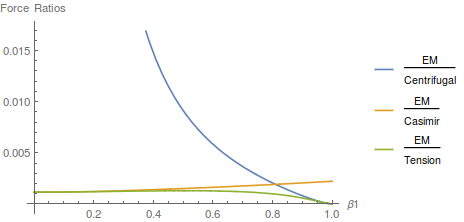
\includegraphics[scale=0.7]{figures/VerifyEMApprox.png}
\caption{Ratios of electromagnetic force to other forces for realistic parameters. Note the casimir force is included, as explained later.}
\label{fig:EMApproxVerify}
\end{figure}

\begin{figure}[h]
\centering
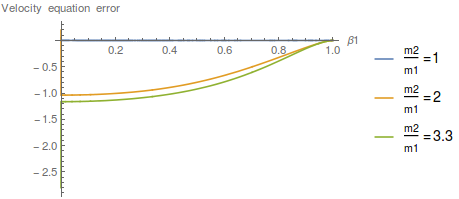
\includegraphics[scale=0.7]{figures/VerifyEMApproxVelocity.png}
\caption{The neglected terms in the velocity relation in units of $m_1\gamma_1^2\beta_1$ for varying mass ratios.}
\label{fig:EMApproxVerifyVelocity}
\end{figure}

%For completeness' sake, we quote the full equation for the velocity relation, including the casimir force which will be explained later:

%\begin{align}
%&\frac{\pi  \tilde{a} \omega }{\sqrt{1-\beta_1^2} (\beta_1+\beta_2)^2}-\frac{\pi  \tilde{a} \omega }{\sqrt{1-\beta_2^2} (\beta_1+\beta_2)^2}+\frac{2 \beta_1 m_1}{\beta_1^2-1}-\frac{2 \beta_2 m_2}{\beta_2^2-1}+ \notag \\
%&+\frac{4 \beta_1^2 \beta_2 q_1 q_2 \omega }{\sqrt{1-\beta_2^2} (\beta_1 \beta_2 \sin (\Delta \theta )+\Delta \theta )^3}-\frac{4 \beta_1 \beta_2^2 q_1 q_2 \omega }{\sqrt{1-\beta_1^2} (\beta_1 \beta_2 \sin (\Delta \theta )+\Delta \theta )^3}+\notag \\
%&+\frac{2 \Delta \theta  q_1 q_2 \omega  \left(\beta_1^2 (-\beta_2) \sqrt{1-\beta_2^2}+\sqrt{1-\beta_1^2} \beta_1 \left(\beta_2^2+1\right)-\beta_2 \sqrt{1-\beta_2^2}\right) \sin (\Delta \theta )}{\sqrt{1-\beta_1^2} \sqrt{1-\beta_2^2} (\beta_1 \beta_2 \sin (\Delta \theta )+\Delta \theta )^3}+\notag \\
%&+\frac{2 \beta_1^2 \beta_2^3 q_1 q_2 \omega }{\sqrt{1-\beta_2^2} (\beta_1 \beta_2 \sin (\Delta \theta )+\Delta \theta )^3}-\frac{2 \beta_1 q_1 q_2 \omega }{\sqrt{1-\beta_1^2} (\beta_1 \beta_2 \sin (\Delta \theta )+\Delta \theta )^3}-\frac{2 \beta_1^3 \beta_2^2 q_1 q_2 \omega }{\sqrt{1-\beta_1^2} (\beta_1 \beta_2 \sin (\Delta \theta )+\Delta \theta )^3}+\notag \\
%&+\frac{2 q_1 q_2 \omega  \left(-\beta_1^2 \beta_2 \sqrt{1-\beta_2^2} \left(\beta_2^2+2\right)+\sqrt{1-\beta_1^2} \beta_1 \left(2 \beta_2^2+1\right)+\sqrt{1-\beta_1^2} \beta_1^3 \beta_2^2-\beta_2 \sqrt{1-\beta_2^2}\right) \cos (\Delta \theta )}{\sqrt{1-\beta_1^2} \sqrt{1-\beta_2^2} (\beta_1 \beta_2 \sin (\Delta \theta )+\Delta \theta )^3}+\notag \\
%&+\frac{2 \beta_2 q_1 q_2 \omega }{\sqrt{1-\beta_2^2} (\beta_1 \beta_2 \sin (\Delta \theta )+\Delta \theta )^3}=0
%\end{align}

\FloatBarrier
\subsubsection{String Equations}
 
We wish to verify that the spinning string ansatz \ref{eq:SpinningStringAnsatz} is truly a solution to the equations of motion.

Using the following derivatives:
\begin{align*}
&\frac{\partial\mathcal{L}}{\partial(\partial_{\tau}x^{\mu})}=\frac{\partial\mathcal{L}}{\partial u^{\mu}}=-T\cfrac{V_{\mu}\left(u\cdot V\right)-u_{\mu}V^{2}}{\sqrt{\left(u\cdot V\right)^{2}-u^{2}V^{2}}}\\
&\frac{\partial\mathcal{L}}{\partial(\partial_{\sigma}x^{\mu})}=\frac{\partial\mathcal{L}}{\partial V^{\mu}}=-T\cfrac{u_{\mu}\left(u\cdot V\right)-u^{2}V_{\mu}}{\sqrt{\left(u\cdot V\right)^{2}-u^{2}V^{2}}}
\end{align*} 

The equation of motion \ref{eq:eulerfield} is then:
\begin{equation*}
-\partial_{\tau}\left(-T\cfrac{V_{\mu}\left(u\cdot V\right)-u_{\mu}V^{2}}{\sqrt{\left(u\cdot V\right)^{2}-u^{2}V^{2}}}\right)-\partial_{\sigma}\left(-T\cfrac{u_{\mu}\left(u\cdot V\right)-u^{2}V_{\mu}}{\sqrt{\left(u\cdot V\right)^{2}-u^{2}V^{2}}}\right)=0
\end{equation*}

Putting in the spinning string solution \ref{eq:SpinningStringAnsatz} we get
\begin{align*}
&\cfrac{-\partial_{\tau}u_{\mu}}{\sqrt{1-\omega^{2}\sigma^{2}}}+\cfrac{-\omega^{2}\sigma}{\sqrt{1-\omega^{2}\sigma^{2}}}V_{\mu}+\sqrt{1-\omega^{2}\sigma^{2}}\partial_{\sigma}V_{\mu}=0\\
&-\partial_{\tau}u_{\mu}-\omega^{2}\sigma V_{\mu}+\left(1-\omega^{2}\sigma^{2}\right)\partial_{\sigma}V_{\mu}=0
\end{align*} 

The timelike equation is trivially satisfied $\left(V_{0}=\partial_{\tau}u_{0}=0\right)$. In the spatial components, for example $\mu=1$, we get:
\begin{equation*}
\omega^{2}\sigma cos\left(\omega\tau\right)
+\omega^{2}\sigma cos\left(\omega\tau\right)
-\left(1-\omega^{2}\sigma^{2}\right)\partial_{\sigma}cos\left(\omega\tau\right)=0
\end{equation*}
Which demonstrates the equations are satisfied.
\FloatBarrier
 \subsection{Energy}
 
 Calculating the energy can be done in two ways. Either as the generator of poincare time translations, or as the hamiltonian of the gauge fixed system. We show the second choice here:
\begin{align*}
E&=\int d\sigma\left(\cfrac{\partial\mathcal{L}}{\partial\dot{\theta}}\dot{\theta}-\mathcal{L}\right)+\cfrac{\partial L}{\partial\dot{\theta}}\dot{\theta}-L \\
&=T\int_{-l_{2}}^{l_{1}}d\sigma\cfrac{1+\sigma^{2}\theta'^{2}}{\sqrt{1+\sigma^{2}\left(\theta'^{2}-\dot{\theta}^{2}\right)}}+m\cfrac{1}{\sqrt{1-\sigma^{2}\dot{\theta}^{2}}}|_{\sigma=-l_{2}}^{\sigma=l_{1}}+q_{1}A^{t}\left(l_{1}\right)
\end{align*} 

Notice in the electromagnetic part we took just one contribution out of the two end points. This is because it already contains the coloumb interaction energy, and taking both “contibutions” would constitute taking it twice.

Inserting the spinning string solution \ref{eq:SpinningStringAnsatz} and electromagnetic potential \ref{eq:fields} we get
\begin{align}
E&=T\int_{-l_{2}}^{l_{1}}d\sigma\cfrac{1}{\sqrt{1-\omega^{2}\sigma^{2}}}+m\cfrac{1}{\sqrt{1-\sigma^{2}\omega^{2}}}|_{-l_{2}}^{l_{1}}+\frac{q_{1}q_{2}\omega}{\beta_{1}\beta_{2}\sin(\Delta\theta)+\Delta\theta}=\notag\\
&=T\frac{sin^{-1}(\beta_{1})}{\omega}+T\frac{sin^{-1}\left(\beta_{2}\right)}{\omega}+\cfrac{m_{1}}{\sqrt{1-\beta_{1}^{2}}}+\cfrac{m_{2}}{\sqrt{1-\beta_{2}^{2}}}+\frac{q_{1}q_{2}\omega}{\beta_{1}\beta_{2}\sin(\Delta\theta)+\Delta\theta}
\end{align} 
\FloatBarrier
 \subsection{Angular Momentum}
 
 The angular momentum is obtained as the generator of rotations. For the rotations in the rotation plane of the string:
\begin{align*}
J&=\int d\sigma\cfrac{\partial\mathcal{L}}{\partial\dot{\theta}}+\cfrac{\partial L}{\partial\dot{\theta}}=\\
&=T\int_{-l_{2}}^{l_{1}}d\sigma\cfrac{\sigma^{2}\dot{\theta}}{\sqrt{1+\sigma^{2}\left(\theta'^{2}-\dot{\theta}^{2}\right)}}+m_{1}\cfrac{l_{1}^{2}\dot{\theta}}{\sqrt{1-l_{1}^{2}\dot{\theta}^{2}}}+m_{2}\cfrac{l_{2}^{2}\dot{\theta}}{\sqrt{1-l_{2}^{2}\dot{\theta}^{2}}}+q_{1}l_{1}A^{\theta}\left(l_{1}\right)+q_{2}l_{2}A^{\theta}\left(l_{2}\right)
\end{align*} 

Inserting the spinning string solution \ref{eq:SpinningStringAnsatz} and electromagnetic potential \ref{eq:fields} we get
\begin{align}
J&=T\int_{-l_{2}}^{l_{1}}d\sigma\cfrac{\sigma^{2}\omega}{\sqrt{1-\sigma^{2}\omega^{2}}}+m_1\cfrac{l_{1}^{2}\omega}{\sqrt{1-l_{1}^{2}\omega^{2}}}+m_2\cfrac{l_{2}^{2}\omega}{\sqrt{1-l_{2}^{2}\omega^{2}}}+\notag \\
&-q_{1}q_{2}\frac{\beta_{1}\beta_{2}\cos(\Delta\theta)}{\beta_{1}\beta_{2}\sin(\Delta\theta)+\Delta\theta}-q_{1}q_{2}\frac{\beta_{1}\beta_{2}\cos(\Delta\theta)}{\beta_{1}\beta_{2}\sin(\Delta\theta)+\Delta\theta}=\notag\\
&=T\cfrac{-\cfrac{\beta_{1}}{\gamma_{1}}+sin^{-1}\left(\beta_{1}\right)-\cfrac{\beta_{2}}{\gamma_{2}}+sin^{-1}\left(\beta_{2}\right)}{2\omega^{2}}+m_1\cfrac{\gamma_{1}\beta_{1}^{2}}{\omega}+m_2\cfrac{\gamma_{2}\beta_{2}^{2}}{\omega}-q_{1}q_{2}\frac{2\beta_{1}\beta_{2}\cos(\Delta\theta)}{\beta_{1}\beta_{2}\sin(\Delta\theta)+\Delta\theta}
\end{align} 
\FloatBarrier
 \subsection{Regge Trajectories and the Regge Intercept}
 \label{sec:regge}
 
Plotting $\left(J,E^{2}\right)$ as a function of $\beta_{1}$ gives the predicted classical Regge trajectories. In order to account for the observed intercept in the Regge trajectories we can add it in using three methods:
\begin{enumerate}
\item Put an intercept by hand into the angular momentum: $J\rightarrow J+a$
\item Put an intercept by hand into the energy squared: $\alpha'E^{2}\rightarrow\alpha'E^{2}-a$
%\item Introduce a constant repulsive force which induces an intercept.
\item Introduce a casimir energy $E_{casimir}=-\frac{\pi}{2}\frac{\tilde{a}}{L}$ which also induces a force and an intercept.
\end{enumerate}

The first and second methods are the simplest phenomenological ways to introduce an intercept. The first has been used in \cite{Sonnenschein14} and \cite{Sonnenschein15}. The second method was used by us as a warmup exercise and has given identical results. While these are good for an initial assessment of the model by comparing with regge trajectories, they suffer from a number of practical problems. First, there is no clear connection of the intercept and the dynamical mechanism which generated it. Second, the string tends to shrink to zero size, which can be problematic for some $J=0$ states.

The following two subsections describe the analysis of the trajectories in the third and fourth methods above.
%\FloatBarrier
%\subsubsection{Repulsive Force Prescription}

%$T=\frac{q^2}{L^2}+\frac{\sqrt{a/\alpha'}}{L}$
%$E=\frac{q^2}{L}+TL$

%This approach aims to reproduce the effect of the second prescription %($\alpha'E^{2}\rightarrow\alpha'E^{2}-a$) by dynamical means. As we will see, this turns out to have problematic properties. The classical string boundary equation is:
%\begin{equation}
%TL=m\beta^2
%\end{equation}
%Which has the form of the energy 
%\begin{equation}
%E=TL+m\beta^2
%\end{equation}
%Suppose we add a force so that

%\begin{equation}
%T=\frac{m\beta^2}{L}+\frac{\sqrt{a/\alpha'}}{L}
%\end{equation}

%And the energy expression remaines the same. 

%\begin{equation}
%E=2m\beta^2+a\sqrt{T}
%\end{equation}
\FloatBarrier
\subsubsection{Casimir Energy Prescription}
In the last option the induced force is 
\begin{equation}
F_{casimir}=-\frac{d}{dL}E_{casimir}=-\frac{\pi}{2}\frac{\tilde{a}}{L^{2}}
\end{equation}
This force is attractive for $\tilde{a}>0$ and repulsive for $\tilde{a}<0$. Notice this energy term has exactly the form of the quantum correction to the string potential (equation \ref{eq:stringpotential}) induced by the quantum zero mode energy corrections. $\tilde{a}$ paramatrizes the (quark mass dependent) sum over the zero mode frequencies, and turns out to be attractive for the case of zero masses ($\tilde{a}=\frac{\left(D-2\right)}{12}>0$). If the casimir force is repulsive it can prevent the system from collapsing to zero size when there is no spin and the electromagnetic force is attractive (leaving no other force to balance the attraction). So we limit the parameter $\tilde{a}<0$. The force is radial and so does not contribute to angular momentum.

Adding the appropriate terms to the expressions for the energy and boundary equations, the equations for construction of the regge trajectories are then:
\begin{subequations}
\label{eq:regge}
\begin{align}
&E=\cfrac{T}{\omega}\left(\sin^{-1}(\beta_{1})+\sin^{-1}(\beta_{2})\right)+\gamma_{1}m_{1}+\gamma_{2}m_{2}+\frac{q_{1}q_{2}\omega}{\beta_{1}\beta_{2}\sin(\Delta\theta)+\Delta\theta}-\frac{\pi}{2}\frac{\tilde{a}\omega}{\beta_{1}+\beta_{2}}\\
&J=T\cfrac{-\cfrac{\beta_{1}}{\gamma_{1}}+sin^{-1}\left(\beta_{1}\right)-\cfrac{\beta_{2}}{\gamma_{2}}+sin^{-1}\left(\beta_{2}\right)}{2\omega^{2}}+m_{1}\cfrac{\gamma_{1}\beta_{1}^{2}}{\omega}+m_{2}\cfrac{\gamma_{2}\beta_{2}^{2}}{\omega}-2q_{1}q_{2}\beta_{1}\beta_{2}\frac{cos\left(\Delta\theta\right)}{\beta_{1}\beta_{2}sin\left(\Delta\theta\right)+\Delta\theta}\\
&\Delta\theta^{2}=\beta_{1}^{2}+\beta_{2}^{2}+2\beta_{1}\beta_{2}cos\left(\Delta\theta\right)\\
&\gamma_{1}^{2}\beta_{1}m_{1}=\gamma_{2}^{2}\beta_{2}m_{2}\\
&\frac{\pi  \omega ^2 (a-S)}{2 (\beta_1+\beta_2)^2}-\frac{\beta_1 m_1 \omega }{\sqrt{1-\beta_1^2}}+T\sqrt{1-\beta_1^2}+\\
&-q_1 q_2 \omega ^2 \frac{\beta_1 \left(2 \beta_1^2 \beta_2^2+2 \beta_1 \left(\beta_2^2+1\right) \beta_2 \cos (\Delta \theta )+2 \beta_1 \beta_2 \Delta \theta  \sin (\Delta \theta )+3 \beta_2^2+2\right)}{2 (\beta_1 \beta_2 \sin (\Delta \theta )+\Delta \theta )^3}+\notag\\
&-q_1 q_2 \omega ^2\frac{\beta_2 \left(\left(\beta_1^2-2 \Delta \theta ^2+2\right) \cos (\Delta \theta )+\beta_1^2 \cos (\Delta \theta )+\beta_1 \beta_2 \cos (2 \Delta \theta )+2 \Delta \theta  \sin (\Delta \theta )\right)}{2 (\beta_1 \beta_2 \sin (\Delta \theta )+\Delta \theta )^3}=0\notag
\end{align}
\end{subequations}

We can obtain analytic expressions for the regge trajectory in the two following limits:
\begin{itemize}
\item $\beta\rightarrow0$: In this limit the quarks are slowly moving, implying most of the energy is related to the string and end points and the quarks are heavy.
\item $\beta\rightarrow1$: In this limit the quarks are relativistic, implying most of the energy is related to the motion and the quarks are light.

\end{itemize}
In both cases we expand the energy and angular momentum around the limit, obtaining series of either $\beta$ or $\left(1-\beta\right)$. From the series for the energy $E=f\left(\beta\right)$ (or $E=f\left(1-\beta\right)$) we calculate the inverse series $\beta=f^{-1}\left(E\right)$ or $1-\beta=f^{-1}\left(E\right)$ .This can then be inserted into the power series for the angular momentum, and obtain the regge trajectory $J\left(E\right)$. This process is automated using computer algebra systems (Mathematica in our case). The code is shown in section \ref{sec:analytic}.

The parameter $\tilde{a}$ is related in the heavy quark limit to the spin $S$ of the quarks. Taking the limit $\beta\rightarrow0$ we get the following energy, angular momentum and force equations (where $L$ is the string length):
\begin{subequations}
\label{eq:nonrelativistic}
\begin{align}
&E=TL+m_{1}+m_{2}+\frac{q_1q_2-\frac{\pi}{2}\tilde{a}}{L}\\ 
&J=0\\
&\frac{q_1q_2-\frac{\pi}{2}\tilde{a}}{L^{2}}=T
\end{align}
\end{subequations}
See appendix \ref{sec:nonrelativistic} for details of the derivation.
Putting the two together we get
\begin{subequations}
\begin{align}
&E=2\sqrt{T}\sqrt{q_1q_2-\frac{\pi}{2}\tilde{a}}+m_1+m_2\label{eq:nonrelativistic2}\\
&\text{Which is equivalent to:}\notag\\
&\alpha'\left(E-m_{1}-m_{2}\right)^{2}-\frac{2}{\pi}q_1q_2+\tilde{a}=0
\end{align}
\end{subequations} 
Noting that the Regge trajectories have the form $J=\alpha'E^2+a$ (neglecting the charge contribution) and using the fact that $J=J_{orbital}\pm S$:
\begin{align}
&J-a=-\tilde{a}=J_{orbital}\pm S-a\\
&J_{orbital}=a\mp S-\tilde{a}
\end{align}
Now because $\beta=0$ then $J_{orbital}=0$ so that
\begin{equation}
\label{eq:atilde}
\tilde{a}=a\mp S
\end{equation}
We also see that $a$ is indeed an intercept in the nonrelativistic (massive quarks) limit, and that the electromagnetic interaction contributes an intercept as well.

In section \ref{sec:reggefit} we present the numerical fits to PDG data, and determine values for the slope and endpoint masses. It is also beneficial to obtain analytic expressions for the regge trajectories, which we can compare with the corresponding expressions for the uncharged model, as well as see what is the effect of the charge on the trajectory. That is the purpose of the next two sections, which present the results at leading order in two limits.
\FloatBarrier 
\subsubsection{Light Quark Limit}

In this limit the quark velocity is large, $\beta=1-\epsilon^{2}$, $\epsilon\rightarrow0$.
The result when adding massive end points is:
\begin{subequations}
\label{eq:reggeAnalyticLight}
\begin{align}
J&=\alpha' E^2\left(1-\frac{4\sqrt{\pi}}{3}\left(\frac{1}{E}\right)^{3/2}\left(m_{1}^{3/2}+m_{2}^{3/2}\right)+\frac{1}{5}\pi^{3/2}\left(\frac{1}{E}\right)^{5/2}\left(m_{1}^{5/2}+m_{2}^{5/2}\right)\right)\notag\\
&+O\left(\frac{1}{E}\right)^{3}\\
&\text{The result when adding casimir forces and charges as well is:}\notag\\
J&=\frac{1}{4}\pi\tilde{a}-0.479 q_1q_2+\alpha' E^2-\frac{1}{3}4 \sqrt{\pi }  \left(m_1^{3/2}+m_2^{3/2}\right)\alpha'\sqrt{E}+\frac{\pi^{3/2}\alpha' \left(m_1^{5/2}+m_2^{5/2}\right)}{5 \sqrt{E}}
\end{align}
\end{subequations}
\FloatBarrier 
 \subsubsection{Heavy Quark Limit}
 
In this limit the quark velocity is small, $\beta\rightarrow0$. The equations are solved in the same manner. The result when adding massive end points and no charge and casimir is:
\begin{subequations}
\label{eq:reggeAnalyticHeavy}
\begin{align}
J&=\frac{4}{3}\sqrt{\frac{2}{3}}\pi\alpha'\sqrt{\frac{m_{1}m_{2}}{m_{1}+m_{2}}}(E-m_{1}-m_{2})^{3/2}+\frac{7\sqrt{\frac{2}{3}}\pi\alpha'\left(m_{1}^{2}-m_{1}m_{2}+m_{2}^{2}\right)(E-m_{1}-m_{2})^{5/2}}{27\sqrt{m_{1}m_{2}(m_{1}+m_{2})^{3}}}\notag\\
&+O\left((E-m_{1}-m_{2})^{7/2}\right)\\
&\text{The result for equal masses when adding casimir forces and charges is:}\notag\\
J=&
\frac{\sqrt{\frac{\sqrt{T \left(-\pi\tilde{a}-2 q_1q_2\right)}}{36 m \sqrt{T \left(-\pi\tilde{a}-2 q_1q_2\right)}+3 \sqrt{2} T \left(\pi\tilde{a}-4q_1q_2\right)}} \left(-6 \sqrt{2} m \sqrt{T \left(-\pi\tilde{a}-2 q_1q_2\right)}-\pi\tilde{a} T+10q_1q_2T\right)}{2 T}\times\notag\\ 
&\times\sqrt{E-2m+\sqrt{2}\sqrt{T\left(-\left(\pi\tilde{a}+2q_1q_2\right)\right)}}
+O\left(E-2m+\sqrt{2}\sqrt{T\left(-\left(\pi\tilde{a}+2q_1q_2\right)\right)}\right)^{3/2}
\end{align}
\end{subequations}
\FloatBarrier
 \subsection{Mass Differences}
 \label{sec:massdiff}

\cite{PDGmassdif} Due to confinement quarks are confined inside hadrons and are not observed as physical particles. Quark masses therefore cannot be measured directly and must be calculated indirectly through their influence on hadronic properties. Although we often speak of quark masses in the same terms as masses of the electron or muon, quantitative statements about the value of a quark mass must make careful reference to the particular theoretical model within which it is defined.

Historically, the first determinations of quark masses were performed using quark models. The resulting masses only make sense in the limited context of a particular quark model, and cannot be related to the quark mass parameters of the Standard Model. Nonrelativistic quark models use constituent quark masses, which are of order 350 MeV for the u and d quarks. Constituent quark masses model the effects of dynamical chiral symmetry breaking which drives the hadronic masses $~\Lambda_{QCD}$, and are not related to the quark mass parameters of the QCD Lagrangian. Constituent masses are only defined in the context of a particular hadronic model. 

The QCD Lagrangian has a chiral symmetry in the limit that the quark masses vanish. This symmetry is spontaneously broken by dynamical chiral symmetry breaking, and explicitly broken by the quark masses. The nonperturbative scale of dynamical chiral symmetry breaking, $\Lambda_{\chi}$, is around 1 GeV. It is conventional to call quarks heavy if $m>\Lambda_{\chi}$, so that explicit chiral symmetry breaking dominates (c,b, and t quarks are heavy), and light if $m<\Lambda_{\chi}$ , so that spontaneous chiral symmetry breaking dominates (u,d and s quarks are light). At high energies or short distances, nonperturbative effects, such as chiral symmetry breaking, become small and one can, in principle, determine quark masses by analyzing mass-dependent effects using QCD perturbation theory.

Similarily to the above situation, our model also determines quark masses by matching the model parameters with the desired results for observed hadronic properties. A particularly interesting property is the mass difference between hadrons of differing electromagnetic charge but identical Isospin, Baryon number, angular momentum and parity. It turns out that the difference in the mass of the quarks (which we would call in this case "current quarks" by analogy) can be determined without knowledge of the individual quark masses. This is similiar in spirit to Isospin symmetry breaking where the degeneracy in the proton and neutron masses is broken by the difference in the masses of the u and d quarks.

Electromagnetic mass differences for hadrons are known for states with $J_{orbital}=0$, therefore we first analyze the case of $\beta=0$. In the stationary string (equation \ref{eq:nonrelativistic2}):
\begin{align}
&E=2\sqrt{T}\sqrt{\frac{q_1q_2}{137}-\frac{\pi}{2}\tilde{a}}+m_{1}+m_{2} \\
&J=0
\end{align}
The parameters $\tilde{a}=a\mp S$(equation \ref{eq:atilde}),$T$ are measured from the regge trajectory fits while the spin $S$ is related to the angular momentum and parity:
\begin{align*}
&P_{meson}=\left(-1\right)^{L+1}\\
&P_{baryon}=\left(-1\right)^{L}\\
&J=L\pm S
\end{align*}
 
When the charge is negligible relative to the casimir contribution we can approximate:
\begin{equation*}
E\approx\frac{1}{\sqrt{\alpha'}}\sqrt{-\tilde{a}}+\frac{1}{\pi\sqrt{\alpha'}}\frac{\frac{q_1q_2}{137}}{\sqrt{-\tilde{a}}}+m_1+m_2
\end{equation*}

Taking the difference between masses of hadrons which correspond to differently charged versions of the same particle, for which the parameters $a$,$S$,$\alpha'$ are constants:
\begin{equation*}
\Delta E\approx\frac{1}{137\pi\sqrt{\alpha'}}\frac{\Delta (q_1q_2)}{\sqrt{-\tilde{a}}}+\Delta m_{quarks}
\end{equation*}
 
From the mass difference of the hadrons we can infer mass differences between the quarks themselves. For example the proton and neutron are considered as a quark-diquark system of $\left(ud-u\right)$ and $\left(ud-d\right)$ respectively, and so the end point masses are $m_{u}+m_{d}$ and $2m_{d}$ respectively. Furthermore $q_1q_2$ is calculated as $q_{diquark}q_{quark}$ so that $q_{proton}^{2}=\left(\frac{2}{3}-\frac{1}{3}\right)\frac{2}{3}=\frac{2}{9}
, q_{neutron}^{2}=-\left(\frac{2}{3}-\frac{1}{3}\right)\frac{1}{3}=-\frac{1}{9}$. If the hadron is a superposition of electromagnetic states (i.e. $\frac{1}{\sqrt{2}}\left(\left|u\bar{u}\right\rangle \pm\left|d\bar{d}\right\rangle \right)$) then $q^{2}$ is calculated as the average $q^{2}$.
\begin{align*}
M_{neutron}-M_{proton}&=2m_{d}-m_{d}-m_{u}+\frac{1}{137\pi\sqrt{\alpha'}}\frac{\left(-\frac{3}{9}\right)}{\sqrt{-\tilde{a}}}=\\
&=m_{d}-m_{u}+\frac{1}{137\pi\sqrt{\alpha'}}\frac{\left(-\frac{3}{9}\right)}{\sqrt{-\tilde{a}}}
\end{align*}

Reversing the argument, the difference in the quark masses can be calculated from the hadron mass differences and the fit to the regge trajectory:
\begin{equation*}
m_{d}-m_{u}=M_{neutron}-M_{proton}+\frac{1}{137\pi\sqrt{\alpha'}}\frac{\left(\frac{3}{9}\right)}{\sqrt{-\tilde{a}}}
\end{equation*} 
Notice that this calculation does not involve the masses of the $u$ and $d$ quarks, so knowing them explicitly is not required. The slope and casimir term $a$ are put in from the regge fits, so there is some implicit dependence on the endpoint masses. Also when dealing with baryons there is an ambiguity as of what quark and diquark to consider as lying at the ends of the string. The diquark charge is the sum of the charges of the quarks it is composed of, and the ambiguity consists of which quarks are chosen to form the diquark. In the calculations on section \ref{sec:massdiff} we have eliminated this ambiguity by choosing that whenever possible, a diquark would be composed of oppositely charged quarks. This has the physical motivation that oppositely charged quarks should tend to form diquarks more that same charged ones.

The quark mass differences depend crucially on the casimir coefficient and the hadron masses. When extracting the coefficient from the regge trajectories there is an implicit connection between the endpoint masses and the extracted casimir coefficient, but due to the large uncertainty in the endpoint masses there is also a large uncertainty in the casimir coefficient. On the other hand we can record the range of permitted coefficients and masses at some slope $\alpha'$ and input those into the calculation of the mass differences to get a corresponding range of mass differences for each hadron. Comparing the mass differences of $u/d$ quarks between different hadrons should give consistent results (because the location of a flavor brane cannot depend on what kind of hadron one considers). The hope is that the range of consistent quark mass differences would be small, enabling a precise determination of the corresponding quark masses and casimir coefficients. Therefore it is expected that a consistent calculation of mass differences would place more strict bounds on the endpoint masses and the casimir coefficient.

Once the quark mass differences are determined we can make predictions for hadronic electromagnetic mass differences for the states with $J_{orbital}\neq 0$ using equations \ref{eq:regge}.This assumes the intercept does not depend on the rate of rotation. The calculation can be done numerically. Note that in this case the hadronic mass differences will generically depend on the absolute masses of the quarks instead of just their mass differences.

In section \ref{sec:confrontmassdiff} we present the results of the calculation of the up/down mass difference for several different hadrons using the parameters consistent with the regge fits, and analyse the results.

\FloatBarrier
\section{Confronting with PDG Data}

\subsection{Regge Trajectories}
\label{sec:reggefit}

Using the methods outlined in the previous section, we fit the regge trajectories of our model to PDG data for the hadrons. We assume $m_{1}=m_{2}=m$ and generalise using the relation $2m^{3/2}=m_1^{3/2}+m_2^{3/2}$ that holds in the leading order as can be seen from equation \ref{eq:reggeAnalyticLight} and the fits done in \cite{Sonnenschein14} which demonstrate this. Also we take $\alpha_{e}=\frac{1}{137}$.

In previous work \cite{Sonnenschein14,Sonnenschein15} the model with no electric charge was confronted with PDG data. There the intercept was introduced by adding a constant to the angular momentum (method 1 discussed in section \ref{sec:regge}). When done in such a way, there is no way of distinguishing between fits to the total angular momentum $J$ of a hadron, and fits to the orbital angular momentum $J_{orbital}$, of the same hadron, as the intercept could always be adjusted to give either plot. However when introducing an intercept using the casimir energy prescription we can clearly distinguish between the two fits. We find that we cannot fit the model to the total angular momentum $J$ of the hadron. Examples for the $\rho$ and $K^{*}$ mesons can be seen in figure \ref{fig:jfit}. The reason is that the casimir coefficient must be \emph{repulsive} in order for the hadron to be stable at the limit where it is not spinning. As was mentioned in section \ref{sec:regge} this is satisfied when $\tilde{a}<0$. Under this limitation we cannot bring the trajectory to fit in the $J$ plane. However when we plot the same trajectory in the $\left(L,M^2\right)$ plane this intercept disappears: it is just the difference between $J$ and $L$. Therefore, all the fits will be done for $\left(L,E^{2}\right)$.

\begin{figure}[h]
\centering
	\subfloat[$\rho$ J fit]{
	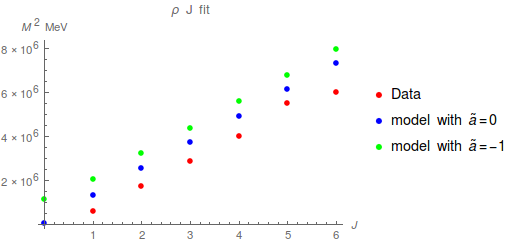
\includegraphics[scale=0.5]{figures/Jtrajectoryrho.png}}
	~
	\subfloat[$K^{*}$ J fit]{
	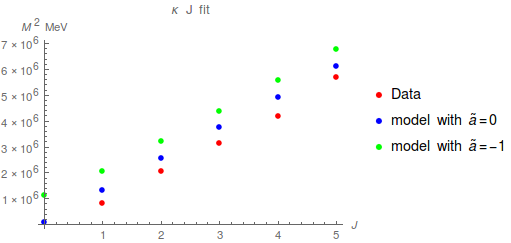
\includegraphics[scale=0.5]{figures/JtrajectoryK.png}}
	\caption{Fits to $\left(J,E^{2}\right)$ for the $\rho$ and $K^{*}$.}
	\label{fig:jfit}  
\end{figure}
 
In the following, we will present the goodness of the fit in the parameter space $\left(m,\alpha'\right)$, and determine values for the universal string tension and end point masses for various hadrons. The fits were done numericaly in Mathematica 10. The goodness of fit is measured in terms of the dimensionless quantity:
\begin{equation}
\label{eq:chisq}
\chi^{2}=\frac{1}{N}\sum_{i\in trajectory}\left(\cfrac{M_{i,pdg}^{2}-M_{i,model}^{2}}{M_{i,pdg}^{2}}\right)^{2}
\end{equation}
$M_{i,model}^{2},M_{i,pdg}^{2}$ are the measured and calculated masses squared of the i-th particle in the trajectory. This quantity is calculated for any given fit. It is then used to compare different fits, with the linear fit as a reference. Figures \ref{fig:mesonfits1},\ref{fig:mesonfits2},\ref{fig:baryonfits} show the mass symmetric fits (endpoint masses assumed to be equal for simplicity),plotting $\frac{\chi^{2}}{\chi_{linear}^{2}}$ as a function of the endpoint masses $m$[MeV] (x-axis) and slope $\alpha'[MeV^{-2}]$ (y-axis). Tables \ref{tab:mesonsum},\ref{tab:baryonsum} are summary tables showing the slope and endpoint masses obtained in the optimal symmetric fit. Tables \ref{tab:mesonsumdorin},\ref{tab:baryonsumdorin} are the corresponding quantities obtained in references \cite{Sonnenschein14} and \cite{Sonnenschein15}.

 \begin{figure}[!h]
 \centering
 	\subfloat[Pion fit]{
 	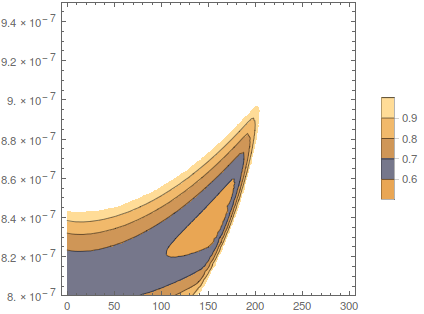
\includegraphics[scale=0.5]{figures/pionFit.png}}
	~
	\subfloat[$\rho$ fit]{
 	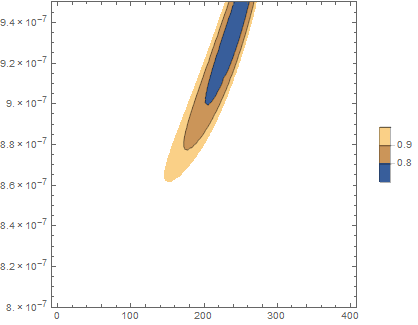
\includegraphics[scale=0.5]{figures/rhoFit.png}}
	
	\subfloat[$\omega$ fit]{
	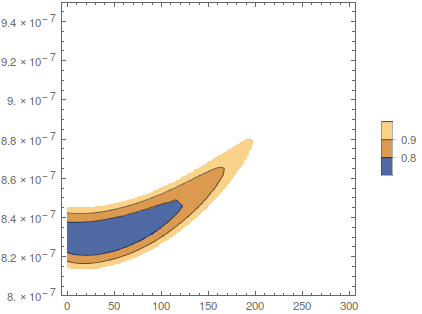
\includegraphics[scale=0.5]{figures/omegaFit.png}}	
	~
	\subfloat[$\eta$ fit]{
	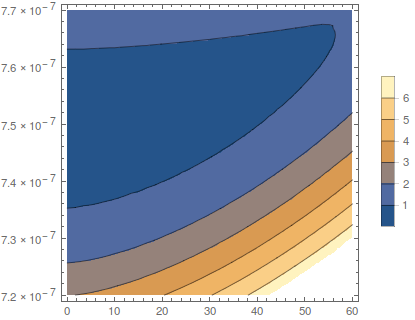
\includegraphics[scale=0.5]{figures/etaFit.png}}
	
	\subfloat[$a_0$ fit]{
	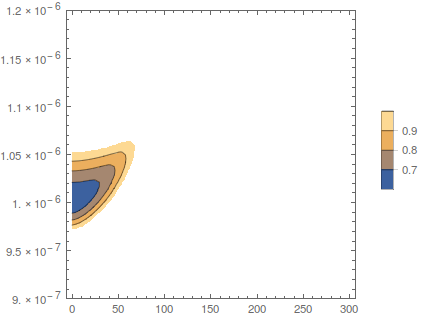
\includegraphics[scale=0.5]{figures/aFit.png}}
	~
	\subfloat[$\theta$ fit]{
	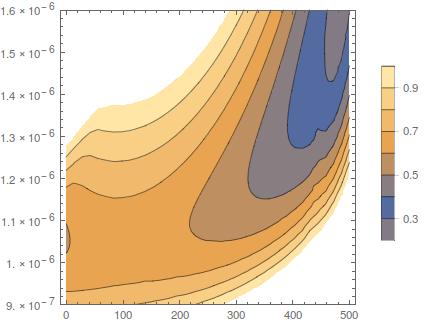
\includegraphics[scale=0.5]{figures/phiFit.png}}
\caption{Meson Fits}
\label{fig:mesonfits1}
\end{figure}

\begin{figure}[!h]
\centering
	\subfloat[$K^*$ fit]{
	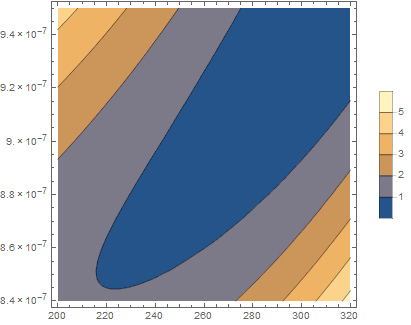
\includegraphics[scale=0.5]{figures/ksFit.png}}
 	~
 	\subfloat[K fit]{
 	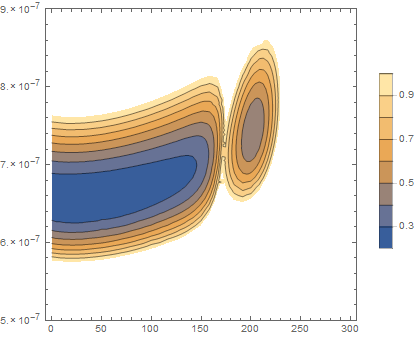
\includegraphics[scale=0.5]{figures/kFit.png}}
 	
 	\subfloat[F fit]{
 	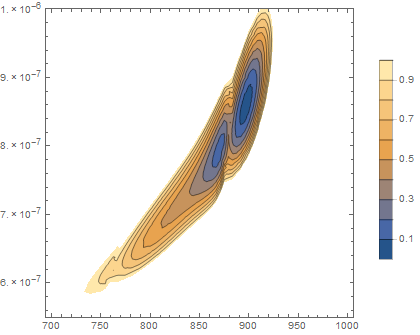
\includegraphics[scale=0.5]{figures/DFit.png}}
 	~
 	\subfloat[B fit]{
 	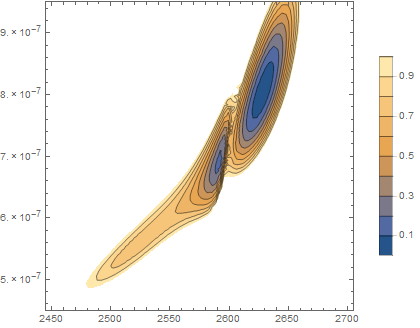
\includegraphics[scale=0.5]{figures/BFit.png}}
 	
 	\subfloat[$\Upsilon$ fit]{
 	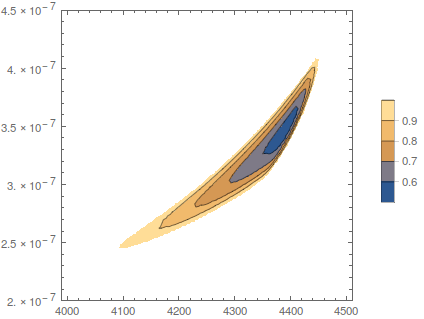
\includegraphics[scale=0.5]{figures/YFit.png}}
\caption{Meson Fits} 
\label{fig:mesonfits2}
\end{figure} 

\begin{figure}[!h]
\centering
 	\subfloat[Proton fit]{
 	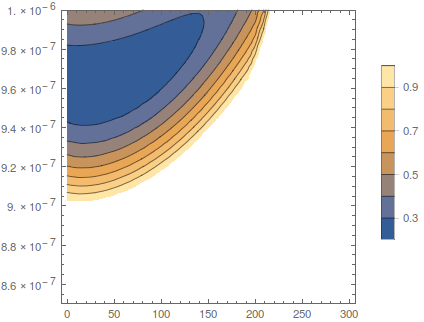
\includegraphics[scale=0.5]{figures/protonFit.png}}
	~
	\subfloat[$\Lambda$ fit]{
	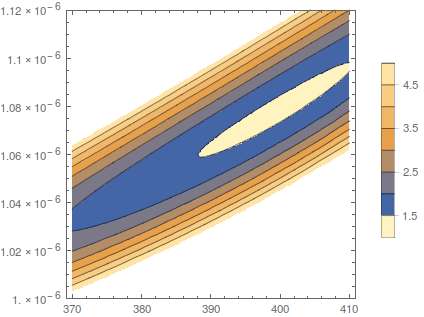
\includegraphics[scale=0.5]{figures/LambdaFit.png}}

 	\subfloat[$\Sigma$ fit]{
 	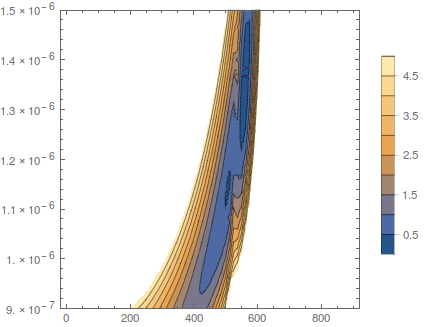
\includegraphics[scale=0.5]{figures/SigmaFit.png}}
	~
	\subfloat[$\Xi$ fit]{
	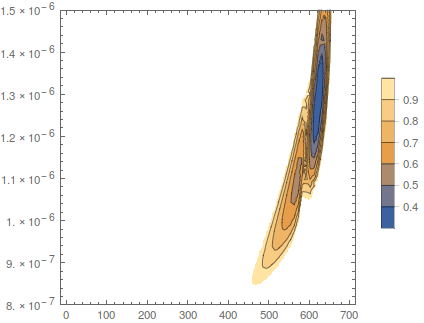
\includegraphics[scale=0.5]{figures/XiFit.png}}
\caption{Baryon Fits}
\label{fig:baryonfits} 
\end{figure}

\begin{table}[h]
\centering
\begin{tabular}{|l|c|c|}
\hline
Hadron & $\alpha '\left[Gev^{-2}\right]$ & Endpoint Masses$\left[MeV\right]$ \\ \hline
$\pi$ & 0.82-0.86 & 100-170 \\
$\rho$  & 0.86-1 & 150-300 \\
$\omega$  & 0.82-0.867 & 0-167 \\
$\eta$  & 0.735-0.765 & 0-60 \\
$a_0$ & 0.97-1.06 & 0-67 \\
$\theta$  & 1.42-1.6 & 450-500 \\
$\kappa$  & 0.95-0.99 & 320-340 \\
$K$ & 0.824-0.95 & 0-200 \\
$D$ & 0.77-0.89 & 860-900 \\
$B$ & 0.8-0.9 & 2630-2650 \\
$\varUpsilon$  & 0.32-0.36 & 4350-4410 \\
\hline
\end{tabular}
\caption{Meson Fits Summary Table}
\label{tab:mesonsum}
%\end{table}

%\begin{table}[h]
\centering
\begin{tabular}{|l|c|c|}
\hline
Hadron & $\alpha '\left[Gev^{-2}\right]$ & Endpoint Masses$\left[MeV\right]$ \\ \hline
$\pi$ & 0.808-0.863 & 90-185 \\
$\rho$  & 0.883-0.933 & 0-180 \\
$\omega$  & 0.910-0.918 & 0-60 \\
$\eta$  & 0.839-0.854 & 0-70 \\
$\theta$  & 1.078 & 400 \\
$\kappa$  & 0.848-0.927 & $m_{u/d}=0-240\; m_s=0-390$ \\
$D$ & 1.073 & $m_{u/d}=80\; m_c=1640$ \\
$\varUpsilon$  & 0.635 & 4730 \\
\hline
\end{tabular}
\caption{Corresponding Meson Fits In \cite{Sonnenschein14}}
\label{tab:mesonsumdorin}
\end{table}

\begin{table}
\centering
\begin{tabular}{|l|c|c|}
\hline
Hadron & $\alpha '\left[Gev^{-2}\right]$ & Endpoint Masses$\left[MeV\right]$ \\ \hline
Proton & 0.94-1 & 0-150 \\
$\Lambda$ & 1.01-1.1 & 385-410 \\
$\Sigma$ & 0.95-1.45 & 400-580 \\
$\Xi$  & 0.84-1.5 & 460-660 \\
\hline
\end{tabular}
\caption{Baryon Fits Summary Table}
\label{tab:baryonsum}
%\end{table}

%\begin{table}
\centering
\begin{tabular}{|l|c|c|}
\hline
Hadron & $\alpha '\left[Gev^{-2}\right]$ & Endpoint Masses$\left[MeV\right]$ \\ \hline
Proton & 0.944-0.959 & 0-85 \\
$\Lambda$ & 0.946-0.955 & 0-62.5 \\
$\Sigma$ & 1.502 & 595 \\
$\Xi$  & 1.455 & 660 \\
\hline
\end{tabular}
\caption{Corresponding Baryon Fits In \cite{Sonnenschein15}}
\label{tab:baryonsumdorin}
\end{table}

We can see that for the most part, the masses obtained in the two kinds of fits are comparable, while the slopes obtained are mostly inconsistent. From our regge fit we can estimate the masses of the various quarks  (see table \ref{tab:quarkmasses}).

\begin{table}
\centering
\begin{tabular}{|l|c|}
\hline
Quark type & Mass range [$MeV$] \\ \hline
u & 150\\ \hline
d & 152.1 \\ \hline
s & 560-601\\ \hline
c & 1331-1396\\ \hline
\end{tabular}
\caption{Estimated quark masses. u/d mass difference is taken from mass difference calculation.}
\label{tab:quarkmasses}
\end{table}

\FloatBarrier
\subsection{Mass Differences}
\label{sec:confrontmassdiff}
We have calculated the mass differences as explained in section \ref{sec:massdiff}, and taken account of the uncertainty in the hadron masses by adding (substracting) it to the maximum (minimum) value of the mass difference. Note that the formula used is \ref{eq:nonrelativistic2} which does not contain any approximation. The data used is shown in table \ref{tab:massdiffdata}. The states   which were chosen could be identified as $J_{orbital}=0$. The results are shown in figure \ref{fig:massdiff}.

As explained in \ref{sec:massdiff} the goal of the calculation requires obtaining a consistent value of the quark mass differences. However, inspecting \ref{fig:massdiff} it is clear that the values thus obtained are not consistent. The most inconsistent values are those obtained from the $K^{*}$ and $D$, while the values for the rest are fairly consistent. 

The inconsistency for the $K^{*}$ is made even more clear by figure \ref{fig:kaonmassdiff} which compares the possible $m_u/m_d$ quark mass differences as a function of the casimir coefficient $a$ (the "intercept"), for the kaon and the neutron/proton. Here it is evident that for most values of the intercept, the obtained mass differences are not consistent. In our case the values (shown in table \ref{tab:massdiffdata} and taken from the Regge fits as previously mentioned) for "a" do not allow for a consistency even if some variation from them is allowed.

The $D$ has an even more puzzling and indeed strange result. Notice the charged $D$ is \emph{heavier} that the neutral $D$ while the situation is reversed for the $K^{*}$. This causes the charge contribution to the quark mass difference in $D$ to have a negative sign. This is compounded by the fact that for the $D$ the value of $\tilde{a}$ extracted from the Regge fit was very small while the values for the observed hadronic mass differences is very small ($M_{D^{+}}-M_{D^{0}}=4.77 MeV$). Overall the calculated mass differences turn out to be negative.

We have not been able to find a mechanism to bring the predicted quark mass differences in agreement. On the other hand it seems that a mass difference of $md-mu=2.1 MeV$ is consistent for most cases.

Taking this mass difference as input (also see tables \ref{tab:mesonsum},\ref{tab:baryonsum}), we can make a prediction of the mass differences of states with higher spin. This is done by calculating the energy of, say, a neutron and a proton at some angular momentum and substracting. The difference in energy of course coming from the different quark masses and charges. Some values are in table \ref{tab:projectedmassdiff}.

\begin{table}
\centering
\begin{tabular}{|l|c|c|c|c|c|c|}
\hline
 Hadron & $\alpha'$ & endpoint mass$\left[MeV\right]$ & $|q_1q_2|$ & $\tilde{a}$ & $S$ \\ 
 \hline
Proton & 0.94 & 938.272 & $\frac{2}{9}$ & \{-1.17,-0.65\} & $\frac{1}{2}$  \\
Neutron & 0.94 & 939.565 & $-\frac{1}{9}$ & \{-1.17,-0.65\} & $\frac{1}{2}$  \\
$\rho^{+}$ & 0.86 & 775.96 & $\frac{2}{9}$ & \{-0.5,-0.1\} & 1  \\
$\rho^{0}$ & 0.86 & 775.26 & $-\frac{5}{18}$ & \{-0.5,-0.1\} & 1  \\
$K^{*+}$ & 0.96 & 889.11 & $\frac{2}{9}$ & \{-0.1,-0.06\} & 1  \\
$K^{*0}$ & 0.96 & 895.81 & $-\frac{1}{9}$ & \{-0.1,-0.06\} & 1  \\
$\Sigma^+$ & 0.95 & 1189.3 & $\frac{2}{9}$ & $\{-0.193513,-0.128062\}$ & $\frac{1}{2}$  \\
$\Sigma^0$ & 0.95 & 1192.6 & $-\frac{1}{9}$ & $\{-0.193513,-0.128062\}$ & $\frac{1}{2}$  \\
$\Xi^0$ & 0.94 & 1314.86 & $-\frac{1}{9}$ & $\{-0.184,-0.035\}$ & $\frac{1}{2}$  \\
$\Xi^-$ & 0.94 & 1321.71 & $\frac{2}{9}$ & $\{-0.184,-0.035\}$ & $\frac{1}{2}$  \\
$D^0$ & 0.86 & 1864.84 & $-\frac{4}{9}$ & $\{-0.14,0\}$ & 1  \\
$D^+$ & 0.86 & 1869.61 & $\frac{2}{9}$ & $\{-0.14,0\}$ & 1  \\
\hline
\end{tabular}
\caption{Slope, Endpoint masses, quark charges and casimir values used in the calculation of the mass differences. Casimir value pairs correspond to values taken for lower and upper limit for mass differences.}
\label{tab:massdiffdata}
\end{table}

\begin{figure}[h]
\centering
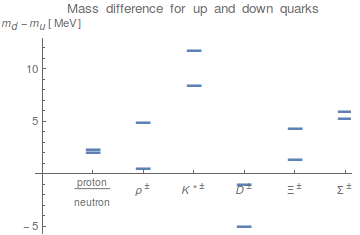
\includegraphics[scale=1]{figures/MassDifferences.png}
\caption{Mass differences between down and up quarks, calculated from various hadrons. For each hadron two values are calculated, each from a different possible value of the casimir term (consistent with the regge fits).}
\label{fig:massdiff}
\end{figure}

\begin{figure}[h]
\centering
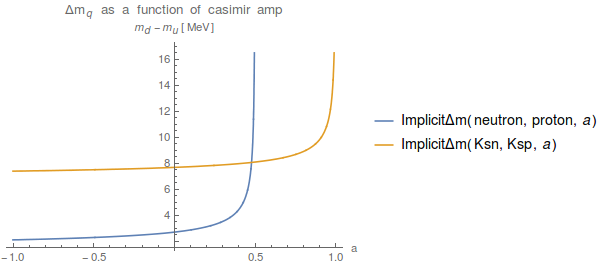
\includegraphics[width=\linewidth]{figures/KaonMassDifferences}
\caption{Mass differences between down and up quarks, calculated from $K^{*\pm}$ vs Proton/Neutron as a function of the "intercept" $a$.}
\label{fig:kaonmassdiff}
\end{figure}

\begin{table}
\centering
\begin{tabular}{|l|c|c|c|}
\hline
\multicolumn{3}{r}{Mass Difference[$MeV$]} \\ \hline
Hadron & L=1 & L=2 & L=3  \\ \hline
$M_{Proton}-M_{neutron}$ & 0.85 & 0.76 & 0.72 \\ \hline
$M_{\Sigma^0}-M_{\Sigma^+}$ & 0.37 & 0.47 & 0.50 \\ \hline
$M_{K^{*n}}-M_{K^{*+}}$ & 0.35 & 0.465 & 0.50 \\ \hline
\end{tabular}
\caption{Projected mass differences for hadrons.}
\label{tab:projectedmassdiff}
\end{table}
\FloatBarrier
\section{Conclusions}

In this thesis we have explored the properties of the charged string with massive ends which corresponds holographicaly to hadrons. By calculating the Regge trajectories we have verified that the electromagnetic interaction contributes an intercept in the Regge trajectories. It is seen that the casimir energy which is generated by quantum fluctuations of the string must induce a repulsive force which keeps the string from collapsing in the case of attractive charges. This same energy consequently contributes another component to the Regge intercept. The resulting model was confronted with PDG data and the model parameters extracted for various hadrons. A new calculation which was attempted is the determination of the u/d mass difference. A mass difference of $2.1 MeV$ is consistent for the hadrons composed of u/d quarks but is not always so when considering hadrons containing more massive quarks.

Upon closer inspection we suspect this is due to the system having some more unusual behaviour in the assymetric masses case. As can be seen from the analysis in section \ref{sec:boundaryequations}, further research is needed to find a better solution of the charged system in the assymetric case. This could change the results of the regge trajectories in the assymetric case and through the change in the parameters also change the mass difference results. Hopefully making all the mass differences consistent. The main difficulty in this direction is the complexity of the underlying equations. One option could be to find a numeric solution to the full equations of motion, but we have not been able to do this to date. Another option would be to perturbatively solve the equations, taking $q_1q_2$ as the small parameter. This is left for future work and is beyond the scope of this thesis.
\appendix
\FloatBarrier
\section{Conventions}
The convention for the metric tensor is the same as in J. D. Jackson 3rd edition (equation 11.59, 11.81):
\begin{equation*}
g_{\mu\nu}=sig(+,-,-,-)
\end{equation*}

And for the electromagnetic field tensor (equations 11.136, 11.137, 11.138):
\begin{equation*}
F^{\alpha\beta}=\left(\begin{array}{cccc}
0 & -E_{1} & -E_{2} & -E_{3}\\
E_{1} & 0 & -B_{3} & B_{2}\\
E_{2} & B_{3} & 0 & -B_{1}\\
E_{3} & -B_{2} & B_{1} & 0
\end{array}\right)
\end{equation*}
\begin{equation*}
F_{\alpha\beta}=\left(\begin{array}{cccc}
0 & E_{1} & E_{2} & E_{3}\\
-E_{1} & 0 & -B_{3} & B_{2}\\
-E_{2} & B_{3} & 0 & -B_{1}\\
-E_{3} & -B_{2} & B_{1} & 0
\end{array}\right)
\end{equation*}
\FloatBarrier
\section{Calculating the electromagnetic fields}
\label{sec:EMFields}

\section{Taking The Nonrelativistic Limit}
\label{sec:nonrelativistic}
In this appendix I will show the manner of taking the nonrelativistic limit in order to arrive at equations \ref{eq:nonrelativistic}.

We start out from equations \ref{eq:regge}, taking the limit $\beta_1\rightarrow0$. We need to determine the $\beta_1$ dependence of the quantities $\beta_2$,$\Delta\theta$ and $\sin\left(\Delta\theta\right)$. 

Determining $\beta_2$ is done using using equation \ref{eq:massrelation}. The form for $\beta_2$ is $\beta_2=a_0+a_1\beta_1+O\left(\beta^3\right)$. Replacing into the equation results in a power series in $\beta_1$ which is equated to zero, so that each coefficient in the series must vanish. This gives equations for the coefficients $\left(a_0,a_1,...\right)$ with the result
\begin{equation*}
\beta_2=\frac{m_1}{m_2}\beta_1+O\left(\beta_1^3\right)
\end{equation*}
Mathematica code for the computation of $\beta_2$:

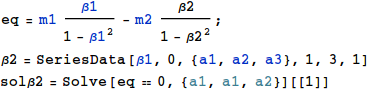
\includegraphics[scale=0.7]{figures/nonrelativisticb2.png}

Using the same method we compute $\Delta\theta$ from equation \ref{eq:retardation}. We put in the solution for $\beta_2$ and get
\begin{equation*}
\Delta\theta=\frac{m_1+m_2}{m_2}\beta_1+O\left(\beta_1^2\right)
\end{equation*}
The solution of $\sin\left(\Delta\theta\right)$ relevant to us is immediate by noting that for $\Delta\theta\rightarrow0$, $\Delta\theta\approx\sin\left(\Delta\theta\right)$.

Mathematica code for the computation of $\Delta\theta$:

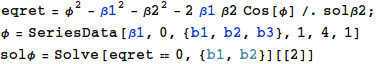
\includegraphics[scale=0.7]{figures/nonrelativisticphi.png}

The final step in obtaining equations \ref{eq:nonrelativistic} is expanding equations \ref{eq:regge} in a taylor series using the two previous results. Mathematica code for the expansion of the energy and force equation:

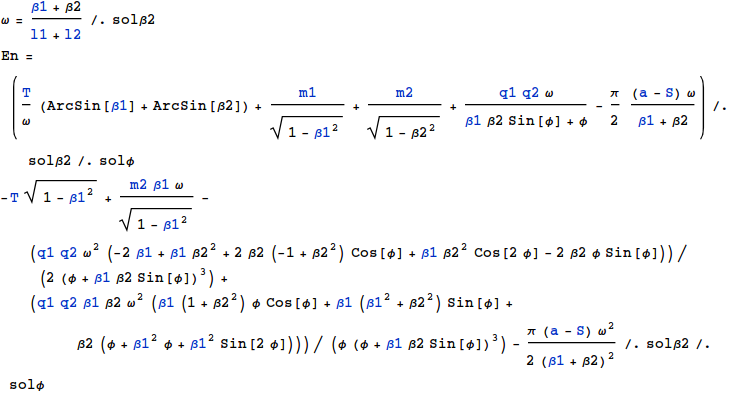
\includegraphics[width=\linewidth]{figures/nonrelativisticeq.png}
This results in the expressions:
\begin{subequations}
\begin{align}
&E=-\frac{\pi}{2}\frac{\tilde{a}}{l_1+l_2}+\frac{q_1 q_2}{l_1+l_2}+T (l_1+l_2)+m_1+m_2\\
&J=0\\
&\frac{q_1 q_2}{(l_1+l_2)^2}-\frac{\pi}{2}\frac{\tilde{a}}{(l_1+l_2)^2}=T
\end{align}
\end{subequations}
Which is what we expected.
\FloatBarrier
\section{Obtaining Analytic Trajectories}
\label{sec:analytic}
\subsection{Relativistic Limit}
The code for obtaining $\beta_2\left(\beta_1\right)$ and $\Delta\theta\left(\beta_1\right)$ (here called $\theta$):

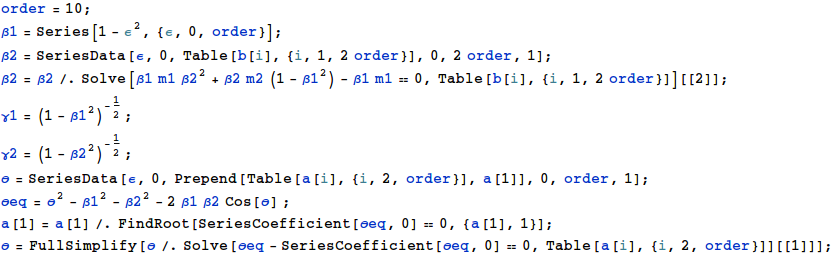
\includegraphics[width=\linewidth]{figures/AnalyticRelativisticKin}

Using that, the code for obtaining the trajectory is:

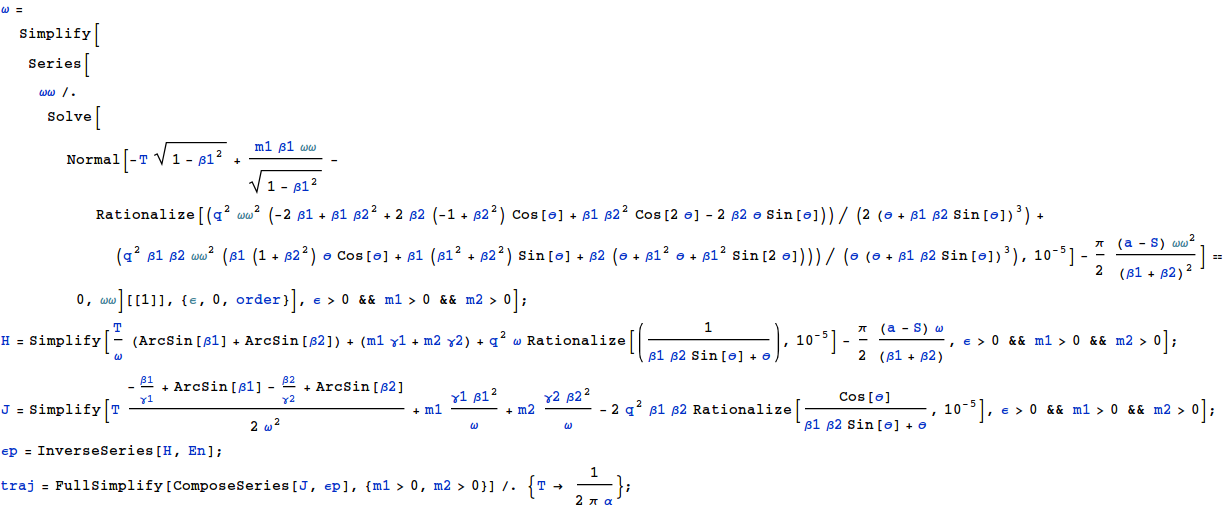
\includegraphics[width=\linewidth]{figures/AnalyticRelativisticRegge}

\subsection{Non Relativistic Limit}
The code for obtaining $\beta_2\left(\beta_1\right)$ and $\Delta\theta\left(\beta_1\right)$ (here called $\theta$):

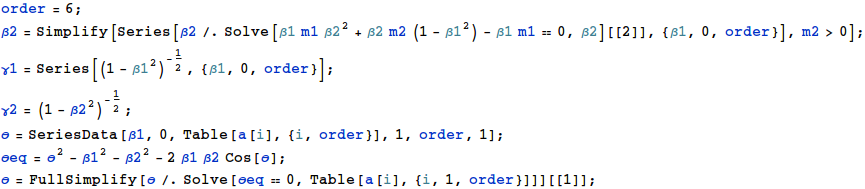
\includegraphics[width=\linewidth]{figures/AnalyticNonRelativisticKin}

Using that, the code for obtaining the trajectory is:

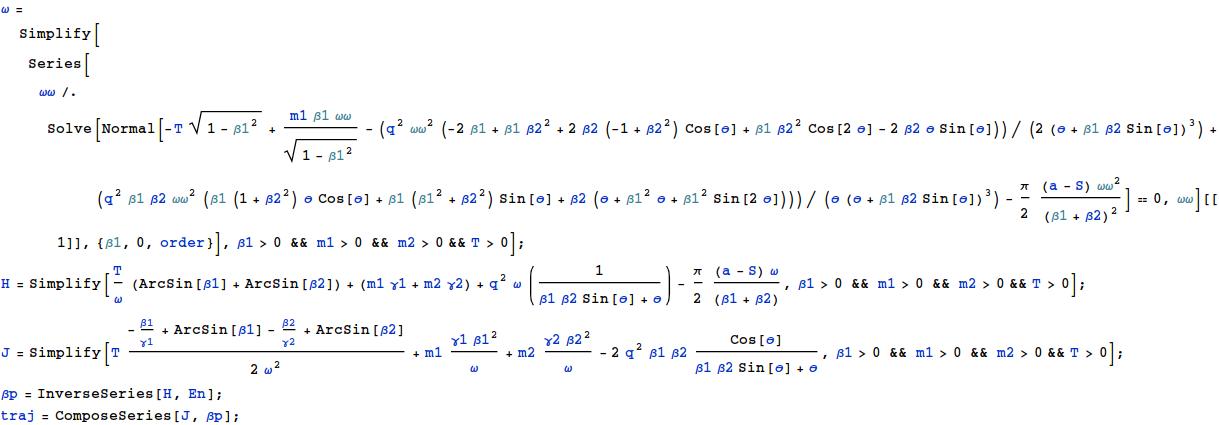
\includegraphics[width=\linewidth]{figures/AnalyticNonRelativisticRegge}
\FloatBarrier
\section{Mass Difference Code}
This appendix documents the Mathematica code used for calculating the mass differences. The data is entered as:

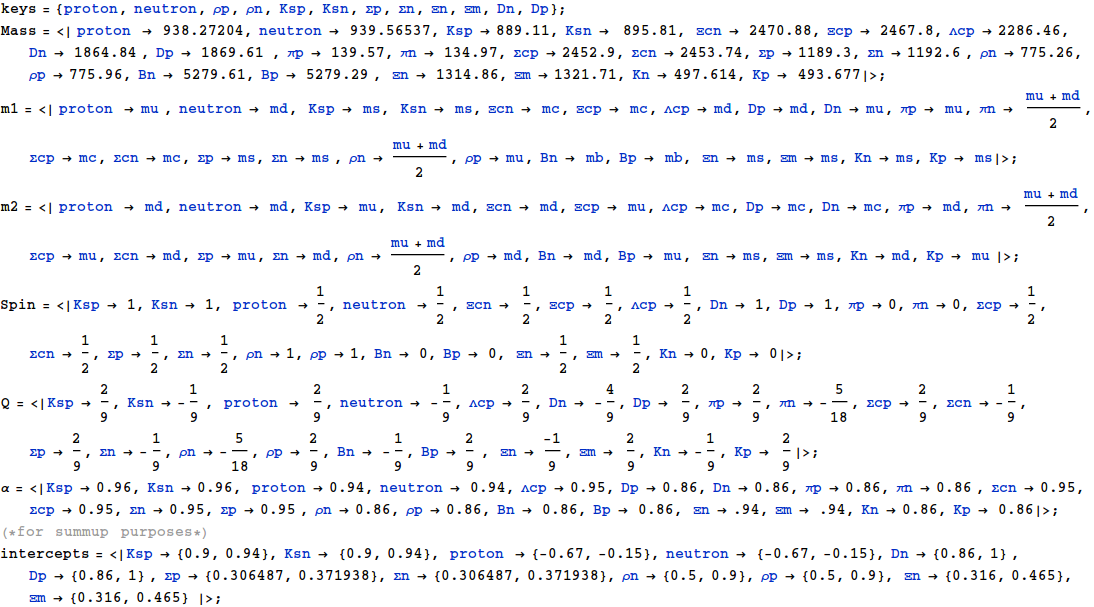
\includegraphics[width=\linewidth]{figures/MassDifferencesData}

The functions used for calculating the mass differences are:

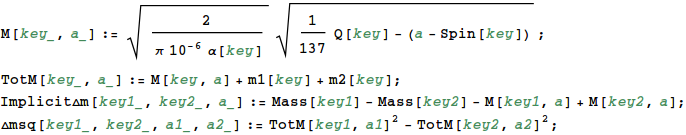
\includegraphics[width=\linewidth]{figures/MassDifferencesFunc}

The code for generating the results is:

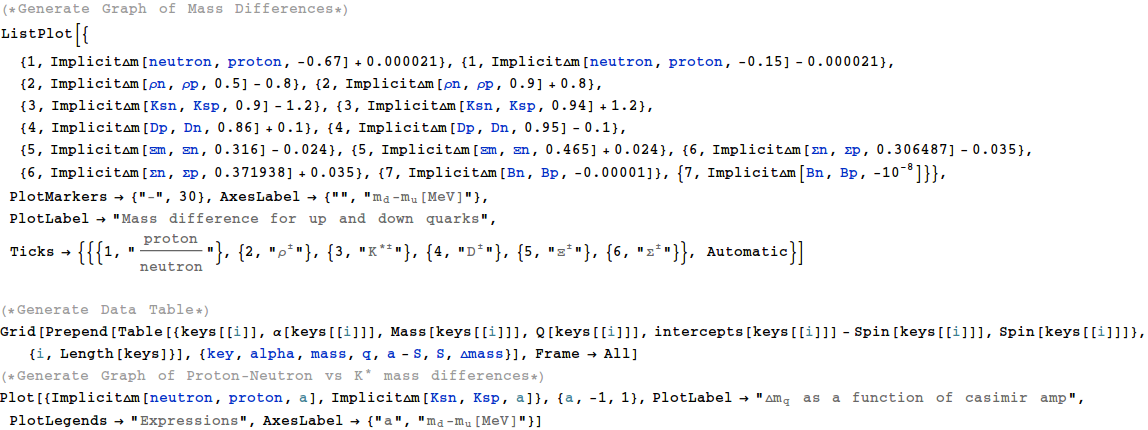
\includegraphics[width=\linewidth]{figures/MassDifferencesCode}

%\bibliographystyle{JHEP}
%\bibliography{Spectrum}

%%%Inline Bibliography
\begin{thebibliography}{9}
\bibitem{Collins}
	P. Collins,
	\emph{An Introduction to Regge Theory and High Energy Physics},
	Cambridge Univeristy
Press,
	1977.
\bibitem{WolframSeriesReversion}
	Weisstein, Eric W,
	\emph{Series Reversion},
	From MathWorld--A Wolfram Web Resource,
	http://mathworld.wolfram.com/SeriesReversion.html
\bibitem{Greensite08}
	J. Greensite,
	\emph{The Confinement Problem in Lattice Gauge Theory},
	Prog.Part.Nucl.Phys. 51 (2003) 1,
	arXiv:hep-lat/0301023v2,
	2003.
\bibitem{Maldacena97}
	Juan Maldacena,
	\emph{The Large N Limit of Superconformal Field Theories and Supergravity},
	Adv.Theor.Math.Phys.2:231-252,1998,
	arXiv:hep-th/9711200v3,
	1997.
\bibitem{Witten98}
	Edward Witten,
	\emph{Anti-de Sitter Space, Thermal Phase Transition, And Confinement In Gauge Theories},
	Adv.Theor.Math.Phys.2:505-532,1998,
	arXiv:hep-th/9803131v2,
	1998.
\bibitem{Kuperstein04}
	S. Kuperstein, J. Sonnenschein,
	\emph{Non-critical, near extremal AdS6 background as a holographic laboratory of four dimensional YM theory},
	JHEP0411:026,2004,
	arXiv:hep-th/0411009v1,
	2004.
\bibitem{Aharony11}
	Ofer Aharony, Steven S. Gubser, Juan Maldacena, Hirosi Ooguri and Yaron Oz,
	\emph{Large N Field Theories, String Theory and Gravity},
	Phys.Rept.323:183-386,2000,
	hep-th/9905111,
	2011.
\bibitem{Vecchia98}
	Paolo Di Vecchia,
	\emph{An introduction to AdS/CFT equivalence},
	Fortsch.Phys.48:87-92,2000,
	arXiv:hep-th/9903007v1,
	1998.
\bibitem{Maldacena98}
	Juan Maldacena,
	\emph{Wilson loops in large N field theories},
	Phys.Rev.Lett. 80 (1998) 4859-4862,
	arXiv:hep-th/9803002v3,
	1998.
\bibitem{Gubser98}
	S.S. Gubser, I.R. Klebanov, A.M. Polyakov,
	\emph{Gauge Theory Correlators from Non-Critical String Theory},
	Phys.Lett.B428:105-114,1998,
	arXiv:hep-th/9802109v2,
	1998.
\bibitem{Sonnenschein00}
	Jacob Sonnenschein,
	\emph{Stringy Confining Wilson Loops},
	Contribution to the Proceedings of the TMR Conference "Non-Perturbative Quantum Effects 2000," Paris, September 2000,
	arXiv:hep-th/0009146v1,
	2000.
\bibitem{Sonnenschein14}
	Jacob Sonnenschein, Dorin Weissman,
	\emph{Rotating strings confronting PDG mesons},
	JHEP 1408 (2014) 013,
	arXiv:1402.5603v3,
	2014.
\bibitem{Sonnenschein15}
	Jacob Sonnenschein, Dorin Weissman,
	\emph{A rotating string model versus baryon spectra},
	JHEP 1502 (2015) 147,
	arXiv:1408.0763v3,
	2015.
\bibitem{Lambiase96}
	G. Lambiase and V. V. Nesterenko,
	\emph{Quark mass correction to the string potential},
	Phys.Rev. D54 (1996) 6387-639,
	1996.
\bibitem{Kinar98}
	Y. Kinar, E. Schreiber, J. Sonnenschein,
	\emph{Q$\bar{Q}$ Potential from Strings in Curved Spacetime - Classical Results},
	Nucl.Phys. B566 (2000) 103-125,
	arXiv:hep-th/9811192v1,
	1998.
\bibitem{Kinar99}
	Y. Kinar, E. Schreiber, J. Sonnenschein, N. Weiss,
	\emph{Quantum fluctuations of Wilson loops from string models},
	Nucl.Phys. B583 (2000) 76-104,
	arXiv:hep-th/9911123v2,
	1999.
\bibitem{Kruczenski05}
	Martin Kruczenski, Leopoldo A. Pando Zayas, J. Sonnenschein, Diana Vaman,
	\emph{Regge Trajectories for Mesons in the Holographic Dual of Large-$N_c$ QCD},
	JHEP0506:046,2005,
	arXiv:hep-th/0410035v2,
	2005.
\bibitem{Jackson}
	J.D. Jackson,
	\emph{Classical Electrodynamics 3rd edition},
	Wiley,
	1998.	
\bibitem{PDG}
	K.A. Olive et al. (Particle Data Group),
	\emph{The Review of Particle Physics},
	Chin. Phys. C, 38, 090001 (2014),
	2015 update.
\bibitem{PDGmassdif}
	A.V. Manohar and C.T. Sachrajda,
	\emph{Quark Masses},
	http://pdg.lbl.gov/2015/reviews/rpp2014-rev-quark-masses.pdf,
	2014 update.	
\bibitem{Sakai04}
	Tadakatsu Sakai, Shigeki Sugimoto,
	\emph{Low energy hadron physics in holographic QCD},
	Prog.Theor.Phys.113:843-882,2005,
	arXiv:hep-th/0412141v5,
	2004.
\bibitem{Seki08}
	Shigenori Seki, Jacob Sonnenschein,
	\emph{Comments on Baryons in Holographic QCD},
	JHEP 0901:053,2009,
	arXiv:0810.1633v3,
	2008.	
	
\end{thebibliography}
\end{document}